% =============================================================================
\section{Introduction}\label{sec:intro}
% =============================================================================

Republic of T\"{u}rkiye stands at a pivotal moment in its transportation electrification trajectory. With 16.2 million registered passenger cars and over one million intercity personal vehicle trips estimated per day on the state highway and motorway system~\cite{tuik_vehicles_2024,kgm_traffic_2024}, road transport accounts for a substantial share of the country's energy consumption and carbon emissions. Recognizing this, T\"{u}rkiye has set ambitious targets for Electric Vehicle (EV) adoption, and the Energy Market Regulatory Authority (EPDK) has licensed a rapidly growing network of public charging stations that now exceeds 9,600 locations operated by more than 170 providers~\cite{sarjgezgini_2025}. Yet the fundamental question facing both policymakers and prospective EV buyers remains unanswered: can this emerging infrastructure support cost-competitive intercity travel, or does the detour and charging time overhead render long-distance EV trips economically impractical compared to conventional Internal Combustion Engine (ICE) vehicles?

Answering this question requires more than aggregate network statistics. It demands a vehicle-level analysis that routes individual trips through the existing charging network, determines where and when each vehicle should stop to recharge, resolves the inevitable conflicts that arise when multiple vehicles converge on the same station, and translates the resulting operational burdens into economic terms. This \textit{scheduling and assessment} perspective is fundamentally different from the \textit{siting} question of where to place new chargers~\cite{kuby_2005,li_2016} or the \textit{sizing} question of how many plugs each station should have~\cite{upchurch_2009,xiong_2024}. While siting and sizing studies prescribe how infrastructure \textit{should} be deployed, a scheduling assessment reveals how well the infrastructure \textit{already deployed} serves the traveling public.

The existing literature on EV charging optimization, reviewed in \cref{sec:lit}, is dominated by studies set in North America and Western Europe, where mature highway networks and established charger registries provide rich input data. Emerging EV markets such as T\"{u}rkiye, where charging networks are growing but unevenly distributed and where intercity distances can be substantial (e.g., over 1,000~km from Istanbul to Diyarbak\i r), have received far less attention. Moreover, most scheduling studies consider individual vehicles or small corridors rather than the millions of trips that define a country-level assessment.

This paper addresses that gap by applying the scalable charging schedule optimization framework of \citet{cokyasar2026electrification}, originally developed and validated for a U.S.\ national-scale analysis, to the full T\"{u}rkiye intercity highway network. The road network is constructed from OpenStreetMap motorway, trunk, and primary road data, yielding a connected graph of 31,286 nodes and 55,236 links. Intercity travel demand is represented by 3 million synthetic origin--destination trips distributed across 100,000 population-weighted locations spanning all 929 districts (\textit{il\c{c}e}) of T\"{u}rkiye. The charging infrastructure comprises 9,641 EPDK-licensed stations drawn from the Sarj Gezgini registry~\cite{sarjgezgini_2025}. The methodological contribution of this paper lies not in the scheduling algorithm itself, which is detailed in~\cite{cokyasar2026electrification}, but in the construction of T\"{u}rkiye-specific inputs, the parametric adaptation to local conditions, and the policy-relevant interpretation of results for an emerging EV market.

The analysis yields several findings of policy relevance. Under a wide State of Charge (SoC) operating window (10--100\%), all intercity trips are feasible across T\"{u}rkiye's charging network, but feasibility collapses to 0.3\% under a conventional 20--80\% window, revealing that infrastructure adequacy depends critically on how much of the battery is usable between stops. EVs are 23--26\% cheaper than ICE vehicles at the operational level under all charger power and capacity scenarios, driven by T\"{u}rkiye's favorable fuel-to-electricity price ratio. At the total cost of ownership level, EVs retain a 10--12\% advantage despite a 40\% purchase price premium. Whether the full system, including infrastructure investment, favors EVs depends on station capacity: the per-trip infrastructure burden is recoverable at 5 plugs per station but not at 50, framing a concrete tradeoff between congestion resilience and cost recovery.

The contributions of this paper are as follows:

\begin{enumerate}
    \item The first countrywide, vehicle-level assessment of intercity EV charging readiness for T\"{u}rkiye, covering the full highway network and nearly 10,000 charging stations at 100\% electrification.

    \item A synthetic but empirically grounded intercity demand model for T\"{u}rkiye, derived from the General Directorate of Highways (KGM) traffic statistics and Turkish Statistical Institute (TURKSTAT, a.k.a. T\"{U}\.{I}K) vehicle registration data, providing 3 million origin--destination trips distributed by district-level population.

    \item An eight-scenario case study crossing four charger power levels with two station capacity assumptions, evaluated through a three-tier economic framework that decomposes the EV-versus-ICE cost differential into energy, detour time, waiting time, vehicle ownership, and infrastructure investment components under T\"{u}rkiye-specific conditions.

    \item A 200-run parametric sensitivity analysis identifying discharge rate (energy efficiency) as the dominant economic lever, followed by EV range, while charger power shows negligible impact at low adoption rates and SoC operating bounds control a binary feasibility cliff.
\end{enumerate}

The remainder of this paper is organized as follows: \Cref{sec:lit}, \Cref{sec:method}, \Cref{sec:results}, and \Cref{sec:conclusion}.

% =============================================================================
\section{Literature Review}\label{sec:lit}
% =============================================================================

Prior work on EV charging spans infrastructure planning, vehicle-level routing, system-level scheduling, and economic evaluation. Rather than repeating a comprehensive survey, the reader is referred to \citet{cokyasar2026electrification} for an extensive treatment, this section highlights the studies most relevant to T\"{u}rkiye's context and identifies the gap that this paper fills. \Cref{tab:litreview} positions representative studies along key dimensions.

\subsection{Infrastructure Planning versus Infrastructure Assessment}

The dominant strand of the EV charging literature treats infrastructure as a decision variable. Flow-refueling location models~\cite{kuby_2005,upchurch_2009} site stations to maximize intercepted traffic; coverage and budget formulations~\cite{frade_2011,li_2016} balance geographic reach against investment cost; and stochastic extensions~\cite{xiong_2024} hedge against demand uncertainty. Recent studies have also addressed electric bus and commercial fleet charging deployment~\cite{BAZARNOVI2025,BAZARNOVI2025583,DAVATGARI2024953,KALEEM2026103403,DAVATGARI2024361}. All of these works answer the question \textit{where should we build?} In contrast, this paper asks \textit{what can we do with what has already been built?}, a diagnostic stance that is especially informative in markets where deployment decisions have already been made but their system-level adequacy has not been evaluated.

\subsection{Scheduling and Capacity at Scale}

At the single-vehicle level, en-route charging reduces to a resource-constrained shortest-path problem, solvable in seconds by dynamic programming~\cite{bagheri_2020,zhang_2018} or robust optimization~\cite{he_2018}. When multiple vehicles share finite plug supply, however, individually optimal plans can collectively violate station capacity. Queuing models~\cite{bae_2015}, discrete-event simulation~\cite{zhang_2019}, and facility-level scheduling~\cite{lee_2020,tang_2016} each address aspects of this coupling but are limited in scale, typically to a single station, corridor, or fleet of tens to hundreds of vehicles. \citet{cokyasar2026electrification} proposed a three-stage framework, infeasibility pruning, per-vehicle DAG-based DP, and an iterative congestion penalty heuristic with FIFO fallback that scales to millions of vehicles across a national network without requiring a commercial solver. The present paper applies that framework to T\"{u}rkiye; the algorithmic contribution resides in~\cite{cokyasar2026electrification}, and the contribution here lies in the data construction, parametric adaptation, and policy analysis for an emerging market.

\subsection{Economic Competitiveness of Long-Distance EV Travel}

Whether EVs can compete with ICE vehicles on long-distance trips is fundamentally an economic question. Fleet-level TCO studies~\cite{hagman_2016} and levelized charger cost analyses~\cite{ledna_2022} provide useful benchmarks but do not capture trip-level heterogeneity in detour burden, charging delay, and route geography. Statistical assessments based on travel surveys~\cite{needell_2016,chakraborty_2019} estimate the share of vehicle-miles serviceable by EVs but do not optimize charging decisions. The framework used here evaluates costs at the individual path level, decomposing the EV--ICE differential into energy, detour time, waiting time, vehicle ownership, and infrastructure amortization with detour and wait costs produced endogenously by the scheduler rather than assumed exogenously.

\subsection{EV Readiness in Emerging Markets}

Large-scale charging analyses have concentrated on North America and Western Europe, where mature registries (e.g., the U.S.\ AFDC, the EU EAFO) and household travel surveys provide input data. Emerging markets face a different landscape: infrastructure is growing but unevenly distributed, public intercity travel data are scarce, and geographic characteristics, T\"{u}rkiye's 68,000 km highway system connecting 81 provinces across two continents~\cite{kgm_traffic_2024}, differ fundamentally from the settings in which existing models have been tested~\cite{iea_2024}. T\"{u}rkiye's charging network, while exceeding 9,600 EPDK-licensed stations across 170 operators~\cite{sarjgezgini_2025}, has evolved around metropolitan corridors, leaving open the question of whether intercity coverage is sufficient. To our knowledge, no prior work has conducted a countrywide, vehicle-level assessment of intercity EV charging readiness for T\"{u}rkiye or any comparable emerging market at the scale presented here.

\begin{table*}[!htb]
\centering
\caption{Positioning of this study relative to representative prior work.}\label{tab:litreview}
\scriptsize
\begin{tabularx}{\textwidth}{>{\raggedright\arraybackslash}X ccc >{\raggedright\arraybackslash}X >{\raggedright\arraybackslash}X >{\raggedright\arraybackslash}X}
\toprule
& \multicolumn{3}{c}{\textbf{Problem}} & \multicolumn{2}{c}{\textbf{Modeling}} & \multicolumn{1}{c}{\textbf{Approach}} \\
\cmidrule(lr){2-4} \cmidrule(lr){5-6} \cmidrule(lr){7-7}
\textbf{Study} & \textbf{SI} & \textbf{ES} & \textbf{MC} & \textbf{Infrastructure} & \textbf{Capacity} & \textbf{Method / Scale} \\
\midrule
\cite{kuby_2005}         & \checkmark & & & Decision variable & None & Flow-refueling LP / Regional \\
\cite{upchurch_2009}     & \checkmark & & & Decision variable & Aggregate & Capacitated LP / Regional \\
\cite{li_2016}           & \checkmark & & & Decision variable & None & Multi-period MIP / State \\
\cite{xiong_2024}        & \checkmark & & & Decision variable & Aggregate & Stochastic MIP / Regional \\
\cite{bagheri_2020}      & & \checkmark & & Fixed & None & Shortest path / Trip \\
\cite{he_2018}           & & \checkmark & & Fixed & None & Robust opt.\ / Corridor \\
\cite{bae_2015}          & & & \checkmark & Fixed & Analytical & M/M/c queuing / Station \\
\cite{lee_2020}          & & \checkmark & \checkmark & Fixed & Explicit & MIP / Facility \\
\cite{tang_2016}         & & & \checkmark & Fixed & Iterative & Dual decomp.\ / Facility \\
\cite{hagman_2016}       & & & & Assumed & --- & TCO accounting / Fleet \\
\cite{ledna_2022}        & & & & Assumed & --- & Levelized cost / Fleet \\
\cite{needell_2016}      & & & & Assumed & --- & Statistical / National \\
\cite{cokyasar2026electrification} & & \checkmark & \checkmark & Fixed (AFDC) & Iterative + FIFO & DAG DP / $\sim$2.7M vehicles, U.S. \\
\midrule
\textbf{This paper} & & \checkmark & \checkmark & \textbf{Fixed (EPDK)} & \textbf{Iterative + FIFO} & \textbf{DAG DP / $\sim$3M trips, T\"{u}rkiye} \\
\bottomrule
\multicolumn{7}{p{0.98\textwidth}}{\emph{SI: Siting/sizing, ES: En-route scheduling, MC: Multi-vehicle/capacity management. LP: linear program, MIP: mixed-integer program, DP: dynamic programming.}}\\
\end{tabularx}
\end{table*}

% =============================================================================
\section{Methodology}\label{sec:method}
% =============================================================================

This section is organized into three subsections: \Cref{sec:framework_summary}, \Cref{sec:data_construction}, and \Cref{sec:economic_framework}.

\subsection{Scheduling Framework Overview}\label{sec:framework_summary}

We employ the three-stage EV charging scheduling framework developed by \citet{cokyasar2026electrification}; the reader is referred to that work for the full mathematical formulation and algorithmic pseudocode. Here we provide a self-contained summary of the elements necessary to understand the T\"{u}rkiye application.

The problem can be described as follows. Consider a fleet of EVs, each assigned a predetermined intercity route through the road network. A route consists of an ordered sequence of directed links, obtained from a static shortest-path computation between the vehicle's origin and destination. Along each route, a set of charging stations with known locations and finite plug counts is available. After traversing a link, a vehicle may choose to detour from the link's endpoint to the geographically nearest charging station, recharge its battery to a target State of Charge (SoC), and return to the same endpoint before continuing. The central scheduling question is: for each vehicle, after which links should it detour to charge? The answer must respect two families of constraints. First, the vehicle's SoC must remain within an operational window $[\underline{S}, \overline{S}]$ at every point along the route, where $\underline{S}$ is the minimum acceptable SoC (a safety buffer against deep discharge) and $\overline{S}$ is the maximum to which the battery is charged at each stop. Second, the number of vehicles simultaneously occupying plugs at any station must not exceed the station's capacity. The objective is to minimize the total cost incurred by all vehicles, comprising the time cost of round-trip detours to and from charging stations and the waiting cost when a vehicle arrives at a station whose plugs are all occupied.

This joint scheduling problem can be formulated as a mixed-integer program (MIP), but the resulting model is computationally intractable at the scale of the T\"{u}rkiye application: with over two million vehicles, routes averaging hundreds of links each, and nearly ten thousand stations, the number of binary decision variables exceeds $10^8$ before capacity-coupling variables are introduced. However, the problem has a key structural property: if station capacity constraints are temporarily ignored, each vehicle's scheduling subproblem becomes independent and can be solved optimally in isolation. The capacity constraint is the sole source of inter-vehicle coupling. This decomposable structure motivates a three-stage solution pipeline (\cref{fig:pipeline}).

\begin{figure}[!ht]
\centering
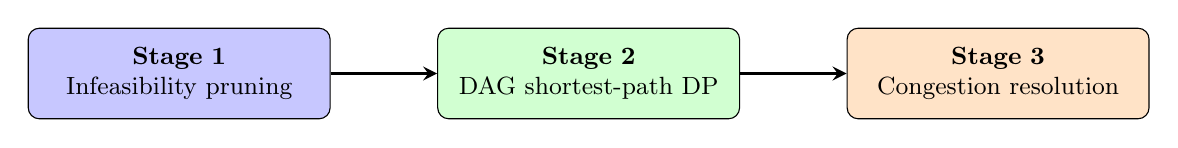
\begin{tikzpicture}[
    box/.style={draw, rounded corners=4pt, minimum width=3.8cm, minimum height=1.15cm,
                text centered, font=\small, fill=#1, text width=3.6cm, text=black},
    arr/.style={->, >=stealth, very thick, black},
]
\node[box=blue!22]   (p1) at (0,   0) {\textbf{Stage 1}\\Infeasibility pruning};
\node[box=green!18]  (p2) at (5.2, 0) {\textbf{Stage 2}\\DAG shortest-path DP};
\node[box=orange!22] (p3) at (10.4,0) {\textbf{Stage 3}\\Congestion resolution};
\draw[arr] (p1.east)--(p2.west);
\draw[arr] (p2.east)--(p3.west);
\end{tikzpicture}
\caption{Three-stage scheduling pipeline from~\cite{cokyasar2026electrification}. DP: Dynamic Programming, DAG: Directed Acyclic Graph.}
\label{fig:pipeline}
\end{figure}

\textbf{Stage~1: Infeasibility Pruning.} Before attempting to optimize charging schedules, the framework identifies vehicles that cannot possibly complete their journey without violating the minimum SoC constraint, regardless of how charging stops are arranged. This occurs when a vehicle's route contains a stretch of consecutive links between two charging opportunities whose cumulative energy consumption exceeds the usable SoC window $\overline{S} - \underline{S}$. A forward-pass reachability heuristic performs this check efficiently by simulating a greedy charging policy along each route: at every link with charger access, it evaluates whether the vehicle has enough remaining SoC to reach the next charger; if not, it charges immediately; if charging is impossible (the charger is unreachable even from the current SoC), the vehicle is declared infeasible and excluded. This pruning step avoids wasting computational resources on vehicles for which no feasible schedule exists.

\textbf{Stage~2: DAG Shortest-Path Solver.} For each surviving vehicle, the framework constructs a Directed Acyclic Graph (DAG) in which nodes represent states defined by a pair: the current link index $i$ along the route and a discretized SoC bucket $s$. The SoC axis is divided into buckets of width $\delta$ (e.g., 1 percentage point), creating $B = \lceil(\overline{S} - \underline{S})/\delta\rceil$ buckets. Two types of arcs connect nodes in consecutive layers. A \textit{travel} arc advances the vehicle to the next link while consuming energy proportional to link distance, at zero monetary cost. A \textit{charge-then-travel} arc represents a detour to the nearest charger, a full recharge to $\overline{S}$, a return to the route, and traversal of the next link, incurring a time-based detour cost. Because the link sequence imposes a strict topological order and SoC transitions are Markovian (the future depends only on the current state, not how the vehicle arrived there), the DAG shortest path from source to any terminal node can be found by a single forward Dynamic Programming (DP) pass in $O(B \cdot N_v)$ time per vehicle, where $N_v$ is the number of links in vehicle $v$'s route. All vehicles are solved independently in parallel across available processor cores.

\textbf{Stage~3: Congestion Penalty Heuristic.} The DAG solver produces individually optimal schedules, but when these are combined across all vehicles, some stations may be assigned more simultaneous users than they have plugs. To resolve these capacity violations, an iterative heuristic augments the DAG arc costs of overloaded stations by a penalty proportional to each station's peak plug overflow (the maximum number of users above capacity across all time bins). Affected vehicles are then re-optimized with the updated costs, which steers them toward less congested alternatives. If improvement stalls, the penalty multiplier is doubled to intensify the pressure. After a fixed number of iterations or a time limit, any remaining capacity violations are resolved by a First-In, First-Out (FIFO) queue simulation that assigns explicit wait times to vehicles arriving at occupied stations. This fallback guarantees that every schedulable vehicle receives a capacity-feasible schedule with a quantified waiting cost.

\subsection{T\"{u}rkiye-Specific Data Construction}\label{sec:data_construction}

Applying the scheduling framework to T\"{u}rkiye required constructing three datasets from scratch: an intercity road network, a synthetic travel demand, and a georeferenced charging station registry. This subsection details each.

The intercity highway network was extracted from OpenStreetMap (OSM) via the Geofabrik regional extract for T\"{u}rkiye. Road segments classified as \texttt{motorway}, \texttt{trunk}, or \texttt{primary} (including their respective \texttt{\_link} variants) were retained; lower-class roads were excluded to restrict the network to intercity-relevant facilities. Segment endpoints within 100 m of each other were merged using a KD-tree spatial snap to create intersection nodes. The largest connected component was retained to ensure full routability, yielding 31,286 nodes and 55,236 directed links. Free-flow speeds were assigned from OSM \texttt{maxspeed} tags where available, with highway-class defaults (motorway: 120 km/h, trunk: 100 km/h, primary: 80 km/h) applied otherwise. All coordinates were projected to EPSG:32636 (UTM Zone 36N). The network was stored as a POLARIS Supply database with proper SpatiaLite geometry infrastructure to enable static shortest-path routing via AequilibraE~\cite{auld_2016}.

No publicly available intercity origin--destination trip table exists for T\"{u}rkiye. We constructed a synthetic demand of 3 million personal vehicle trips representing three days of intercity travel, calibrated to the aggregate volume of approximately one million intercity personal vehicle trips per day reported in KGM traffic statistics~\cite{kgm_traffic_2024}. Origin and destination locations were drawn from 100,000 population-weighted points distributed across all 929 administrative districts (\textit{il\c{c}e}), with district populations derived from T\"{U}\.{I}K census data~\cite{tuik_vehicles_2024} and allocated proportionally using GADM Level 2 boundaries. Trip start times were distributed across three days using an hourly profile that peaks during morning and evening periods. Origins were sampled proportionally to district population; destinations were drawn from a different district to ensure intercity character. All trips were routed through the network using AequilibraE's static shortest-path algorithm, producing link-level trajectories.


Station locations were obtained from the Sarj Gezgini registry~\cite{sarjgezgini_2025}, which aggregates EPDK-licensed public charging stations across T\"{u}rkiye. The dataset contains 9,641 stations operated by 170 networks (largest: ZES with 1,827 stations, E\c{s}arj with 745, Trugo with 649). Geographic coordinates (WGS 84) were projected to EPSG:32636 for consistency with the road network. Because the registry does not report individual plug counts per station, each station was assigned 50 plugs in the baseline scenario (with a 5-plug variant used to assess congestion sensitivity). Station-to-link proximity was computed using a BallTree index with Manhattan distance in projected coordinates.

\subsection{Economic Evaluation Framework}\label{sec:economic_framework}

Following \citet{cokyasar2026electrification}, economic outcomes are evaluated through a three-tier analysis computed at the individual path level and then aggregated. Each tier progressively expands the cost boundary from operational expenses to full system costs. The notation used in the tier equations is as follows. For each vehicle $v$: $D_v$ is the original trip distance (miles), $D_v^{\delta}$ is the total round-trip detour distance (miles) incurred by charging stops, $C_v^{\tau}$ is the total detour time cost (\$), and $C_v^{\omega}$ is the total FIFO waiting cost (\$). Both $C_v^{\tau}$ and $C_v^{\omega}$ are outputs of the scheduling optimization, not assumed parameters. The remaining symbols are shared parameters: $P^{\gamma}$ is the gasoline price (\$/gallon), $P^{\xi}$ is the electricity price (\$/kWh), $\eta^{\gamma}$ is ICE fuel economy (miles per gallon), and $\bar{\rho}$ is the average EV discharge rate (Wh/mile).

Tier~1 (Operational) compares ICE fuel cost against EV electricity, detour, and waiting costs:
\begin{align}
    C_{v}^{\gamma,1} &= \frac{D_v P^{\gamma} }{\eta^{\gamma}} \label{eq:t1ice} \\
    C_{v}^{\xi,1} &= \frac{P^{\xi}(D_v + D_v^{\delta}) \bar{\rho}}{1000} + C_v^{\tau} + C_v^{\omega} \label{eq:t1ev}
\end{align}

Tier~2 (Total Cost of Ownership) adds per-trip vehicle purchase amortization and per-mile maintenance. Let $V^{\gamma}$ denote the ICE vehicle purchase price, $\alpha$ the EV-to-ICE price ratio, $M^{\gamma}$ and $M^{\xi}$ the per-mile maintenance costs for ICE and EV respectively, $F$ the average number of long-distance trips per vehicle per week, and $L$ the vehicle useful life in years:
\begin{align}
    C_{v}^{\gamma,2} &= C_{v}^{\gamma,1} + \frac{V^{\gamma}}{ 52 FL} + M^{\gamma} D_v \label{eq:t2ice} \\
    C_{v}^{\xi,2} &= C_{v}^{\xi,1} + \frac{\alpha V^{\gamma}}{ 52 FL} + M^{\xi} (D_v + D_v^{\delta}) \label{eq:t2ev}
\end{align}

Tier~3 (Infrastructure) adds amortized charging infrastructure capital and operating costs to the EV side. Let $Z^{\text{total}}$ denote the total number of plugs in the network, $\kappa$ the capital cost per plug, $L_c$ the charger useful life in years, $\mu$ the annual operations and maintenance rate as a fraction of capital cost, $\sigma$ the demand sample fraction, and $N^{\text{national}}$ the estimated national vehicle count (obtained by dividing the number of feasible paths by $F$ and scaling by $1/\sigma$):
\begin{align}
    C_{v}^{\xi,3} &= C_{v}^{\xi,2} + \frac{ Z^{\text{total}} (1/L_c + \mu)\kappa}{52FN^{\text{national}}} \label{eq:t3ev}
\end{align}
The ICE cost at Tier~3 is unchanged ($C_{v}^{\gamma,3} = C_{v}^{\gamma,2}$). At each tier, we report both the mean per-path savings percentage, computed as $100 \times (C_{v}^{\gamma,k} - C_{v}^{\xi,k})/C_{v}^{\gamma,k}$ where positive values indicate EVs are cheaper, and the share of individual paths for which the EV is cheaper than ICE.

% =============================================================================
\section{Numerical Experiments}\label{sec:results}
% =============================================================================

\subsection{Experimental Design}\label{sec:design}

The travel demand comprises 3 million synthetic intercity personal vehicle trips representing three days of travel across T\"{u}rkiye, as described in \Cref{sec:data_construction}. All trips are routed through the intercity highway network (31,286 nodes, 55,236 links) using AequilibraE's static shortest-path algorithm, producing link-level trajectories with per-link distances, travel times, and sequences. EV-specific characteristics (range, discharge rate, and starting SoC) are assigned stochastically to each trajectory: range is drawn from a uniform distribution over $[\underline{R}, \overline{R}]$, discharge rate from a triangular distribution with bounds $[\underline{\rho}, \overline{\rho}]$ and mode $\underline{\rho}$, and starting SoC from a triangular distribution with bounds $[\underline{B}, \overline{B}]$ and mode $\overline{B}$.

The charging infrastructure consists of the 9,641 EPDK-licensed stations from the Sarj Gezgini registry~\cite{sarjgezgini_2025}, with each station assigned 50 plugs in the baseline scenario. A single charging network is used for all experiments; the effect of charger technology is examined by varying charger power $W_c$ across four levels (7~kW, 22~kW, 50~kW, and 350~kW) representing slow AC, fast AC, standard DCFC, and ultra-fast DCFC, respectively. A plug-constrained scenario with 5 plugs per station is also considered to assess the sensitivity of congestion outcomes to station capacity. The detour speed $\bar{v}$ governs the time cost of the Manhattan distance detour from a link endpoint to the nearest charger.

\Cref{tab:params} summarizes all parameter values, organized by tier, with their units, baseline values, and references. All monetary values are denominated in Turkish Lira (TL), distances in kilometers, and energy consumption in Wh/km, reflecting T\"{u}rkiye-specific conditions.

\begin{table*}[!htb]
\centering
\footnotesize
\caption{Parameter values used in the experiments.}\label{tab:params}
\begin{tabularx}{\textwidth}{l >{\raggedright\arraybackslash}X l >{\raggedright\arraybackslash}X}
\toprule
\textbf{Symbol} & \textbf{Meaning (unit)} & \textbf{Value / Range} & \textbf{Reference} \\
\midrule
\multicolumn{4}{l}{\textit{Simulation parameters}} \\
$\underline{B},\, \overline{B}$ & Starting SoC bounds (\%) & 80 -- 100 & Assumed \\
$C^\tau$ & Detour cost rate (TL/hr) & 100 & \cite{numbeo_turkey_2025} \\
$C^\omega$ & Waiting cost rate (TL/hr) & 70 & \cite{numbeo_turkey_2025} \\
$\overline{K}$ & Maximum penalty iterations & 15 & -- \\
$\underline{R},\, \overline{R}$ & EV range bounds (km) & 250 -- 550 & \cite{evdatabase_2025} \\
$\underline{S}$, $\overline{S}$ & Operational SoC (\%) bounds & 10 -- 100 & \cite{ev_battery_2022} \\
$W_c$ & Charger power (W) & 350,000 & \cite{zes_pricing_2025} \\
$\delta$ & SoC bucket size (\%) & 1 & -- \\
$\Delta$ & Time bin width (sec) & 900 & -- \\
$\lambda$ & Initial congestion penalty multiplier & 10.0 & -- \\
$\bar{v}$ & Assumed detour speed (km/h) & 90 & Assumed \\
$\underline{\rho},\, \overline{\rho}$ & Discharge rate bounds (Wh/km) & 150 -- 250 & \cite{evdatabase_2025} \\
\midrule
\multicolumn{4}{l}{\textit{Tier~1 economic parameters (operational)}} \\
$P^{\gamma}$ & Gasoline price (TL/liter) & 50.0 & \cite{epdk_gasoline_2025} \\
$P^{\xi}$ & Electricity price (TL/kWh) & 13.0 & \cite{zes_pricing_2025} \\
$\eta^{\gamma}$ & ICE fuel economy (km/liter) & 14.0 & \cite{iea_2024} \\
\midrule
\multicolumn{4}{l}{\textit{Tier~2 economic parameters (total cost of ownership)}} \\
$F$ & Avg.\ long-distance trips per vehicle per week & 3.0 & Assumed \\
$L$ & Vehicle useful life (years) & 13 & \cite{acea_vehicle_age_2024} \\
$M^{\gamma}$ & ICE maintenance cost (TL/km) & 0.35 & \cite{numbeo_turkey_2025} \\
$M^{\xi}$ & EV maintenance cost (TL/km) & 0.12 & \cite{numbeo_turkey_2025} \\
$V^{\gamma}$ & ICE vehicle purchase price (TL) & 2{,}000{,}000 & \cite{numbeo_turkey_2025} \\
$\alpha$ & EV purchase price ratio (EV/ICE) & 1.4 & \cite{eafo_turkey_2025} \\
\midrule
\multicolumn{4}{l}{\textit{Tier~3 economic parameters (infrastructure)}} \\
$L_c$ & Charger useful life (years) & 12 & Assumed \\
$\kappa$ & Charger unit CAPEX (TL/plug) & 1{,}500{,}000 & \cite{iea_2024} \\
$\mu$ & Charger annual O\&M (\% of CAPEX) & 8 & Assumed \\
$\sigma$ & Demand sample fraction & 1.0 & -- \\
\bottomrule
\end{tabularx}
\end{table*}

\Cref{fig:charger_map} shows the geographic distribution of the 9,641 charging stations alongside the intercity highway network. Station density is highest along the Istanbul--Ankara--Izmir triangle and the Mediterranean coastal corridor, with sparser coverage in the eastern provinces. This uneven spatial distribution, which reflects the market-driven rollout of charging infrastructure around major metropolitan demand centers, is a key factor in the feasibility outcomes reported in the case study below.

\begin{figure*}[!htb]
\centering
\includegraphics[width=0.85\textwidth]{turkiye_charger_map.png}
\caption{Geographic distribution of 9,641 EPDK-licensed charging stations (blue triangles) and the intercity highway network (55,236 links, gray lines) across T\"{u}rkiye.}
\label{fig:charger_map}
\end{figure*}

\subsection{Case Study}\label{sec:casestudy}

The case study evaluates the interaction between charger power and station capacity by crossing four power levels (5, 22, 50, and 350~kW) with two plug-count configurations. Because the Sarj Gezgini registry does not report individual plug counts per station, we bracket the unknown capacity with two bounding assumptions: 50 plugs per station (482,050 total plugs), representing an infrastructure-abundant upper bound, and 5 plugs per station (48,205 total plugs), representing a capacity-constrained lower bound. This bracketing approach allows the analysis to characterize the range of possible outcomes rather than relying on a single assumption. All eight scenarios use the same charging network of 9,641 EPDK-licensed stations, the same 3 million synthetic intercity trips, and the full 100\% electrification rate. \Cref{tab:casestudy} reports the key operational and economic metrics. Before discussing the results, it is important to note that several baseline modeling choices distinguish this analysis from the U.S.\ application in \citet{cokyasar2026electrification}: T\"{u}rkiye uses a wider SoC operating window (10--100\% vs.\ 20--80\%), a different charging network (9,641 EPDK stations vs.\ 14,260 AFDC DCFC stations), T\"{u}rkiye-specific fuel and electricity prices (50~TL/liter gasoline, 13~TL/kWh electricity), and a higher EV-to-ICE purchase price ratio (1.4 vs.\ 1.2). These differences affect both feasibility rates and economic outcomes, and direct numerical comparisons between the two studies should be interpreted with this context in mind.

All eight scenarios achieve 100\% feasibility, with all 2,161,247 paths that enter the scheduler completing successfully. This contrasts with the approximately 29\% feasibility rate observed in the U.S.\ analysis, a difference attributable primarily to the wider SoC operating window (10--100\%) rather than to differences in network geography. As demonstrated in \cref{sec:sensitivity}, capping $\overline{S}$ at 80\% collapses feasibility to 0.3\% in the T\"{u}rkiye network, confirming that the full-capacity operating window is the primary enabler of universal feasibility.

Charging operations vary substantially across scenarios. Average charge time per stop ranges from 4.1~minutes at 350~kW to 287--288~minutes at 5~kW, a 70-fold difference that directly impacts vehicle throughput at each station. Average detour time per path ranges from 9.9~minutes (350~kW, 50~plugs) to 23.7~minutes (5~kW, 5~plugs), reflecting the optimizer's preference for more distant but less congested stations when nearby stations have limited capacity. Additional travel distance ranges from 1.7\% to 4.1\% of the original trip distance. The number of charging stops is remarkably stable at approximately 6.1 across all scenarios, indicating that the optimizer selects a similar number of stops regardless of power or capacity, adjusting only the duration and spatial distribution of each stop.

The three-tier economic analysis reveals that EVs are operationally cheaper than ICE vehicles in T\"{u}rkiye under all eight scenarios. Tier~1 (operational) savings range from $+23.2$\% (5~kW, 5~plugs) to $+25.5$\% (350~kW, 50~plugs), and 100\% of individual paths favor EVs at Tier~1 in every scenario. This finding contrasts sharply with the U.S.\ analysis, where Tier~1 savings were negative ($-6.1$\% to $-46.3$\%) across all scenarios. The reversal is driven by T\"{u}rkiye's favorable fuel-to-electricity price ratio: gasoline at 50~TL/liter with 14~km/L efficiency costs approximately 3.57~TL/km, while electricity at 13~TL/kWh with an average discharge rate of 200~Wh/km costs approximately 2.60~TL/km, a 27\% energy cost advantage that absorbs the detour and waiting time overhead.

Tier~2 (TCO) savings narrow to $+10.0$\% to $+11.7$\% as the higher EV purchase price (1.4$\times$ ICE) partially offsets the operational advantage. Approximately 96--97\% of individual paths remain EV-favorable at Tier~2, indicating broad cost competitiveness across trip lengths and geographies.

The plug-count dimension reveals its impact at Tier~3 (Infrastructure), where the total number of plugs determines the amortized infrastructure cost per trip. With 50 plugs per station (482,050 total), the per-trip infrastructure burden overwhelms the Tier~2 advantage, pushing Tier~3 savings to $-15.0$\% to $-15.8$\%. With 5 plugs per station (48,205 total), the infrastructure cost is 10$\times$ lower, and Tier~3 savings remain positive at $+7.4$\% to $+8.0$\%. This Tier~3 sign reversal highlights a fundamental infrastructure planning tradeoff: deploying more plugs per station improves throughput and reduces congestion but increases the per-trip infrastructure burden that must be recovered through charging fees or public subsidy.

\Cref{fig:detour_overhead} illustrates the relationship between trip distance and charging detour overhead for the 350~kW scenario under both plug-count configurations. The overall pattern is consistent: short trips incur proportionally higher detour overhead because a single charging stop represents a larger fraction of the total distance, while detour percentage declines and stabilizes for longer routes. However, the vertical shift between the two panels reveals the impact of station capacity on routing decisions. With 50 plugs per station (median detour overhead 1.5\%), the optimizer selects nearby chargers with minimal deviation from the original path. With 5 plugs per station (median 2.8\%), the optimizer redirects vehicles to more distant but less congested stations, nearly doubling the detour burden. This effect is consistent across all distance bins: for trips over 1,000~km, mean detour overhead increases from 1.9\% (50 plugs) to 3.6\% (5 plugs). The scatter also reveals substantial trip-level heterogeneity in both configurations, with detour overhead varying by a factor of 5--10 at any given distance depending on the specific origin-destination pair and the proximity of the route to available stations.

\begin{figure*}[!htb]
\centering
\begin{subfigure}[t]{0.48\textwidth}
    \centering
    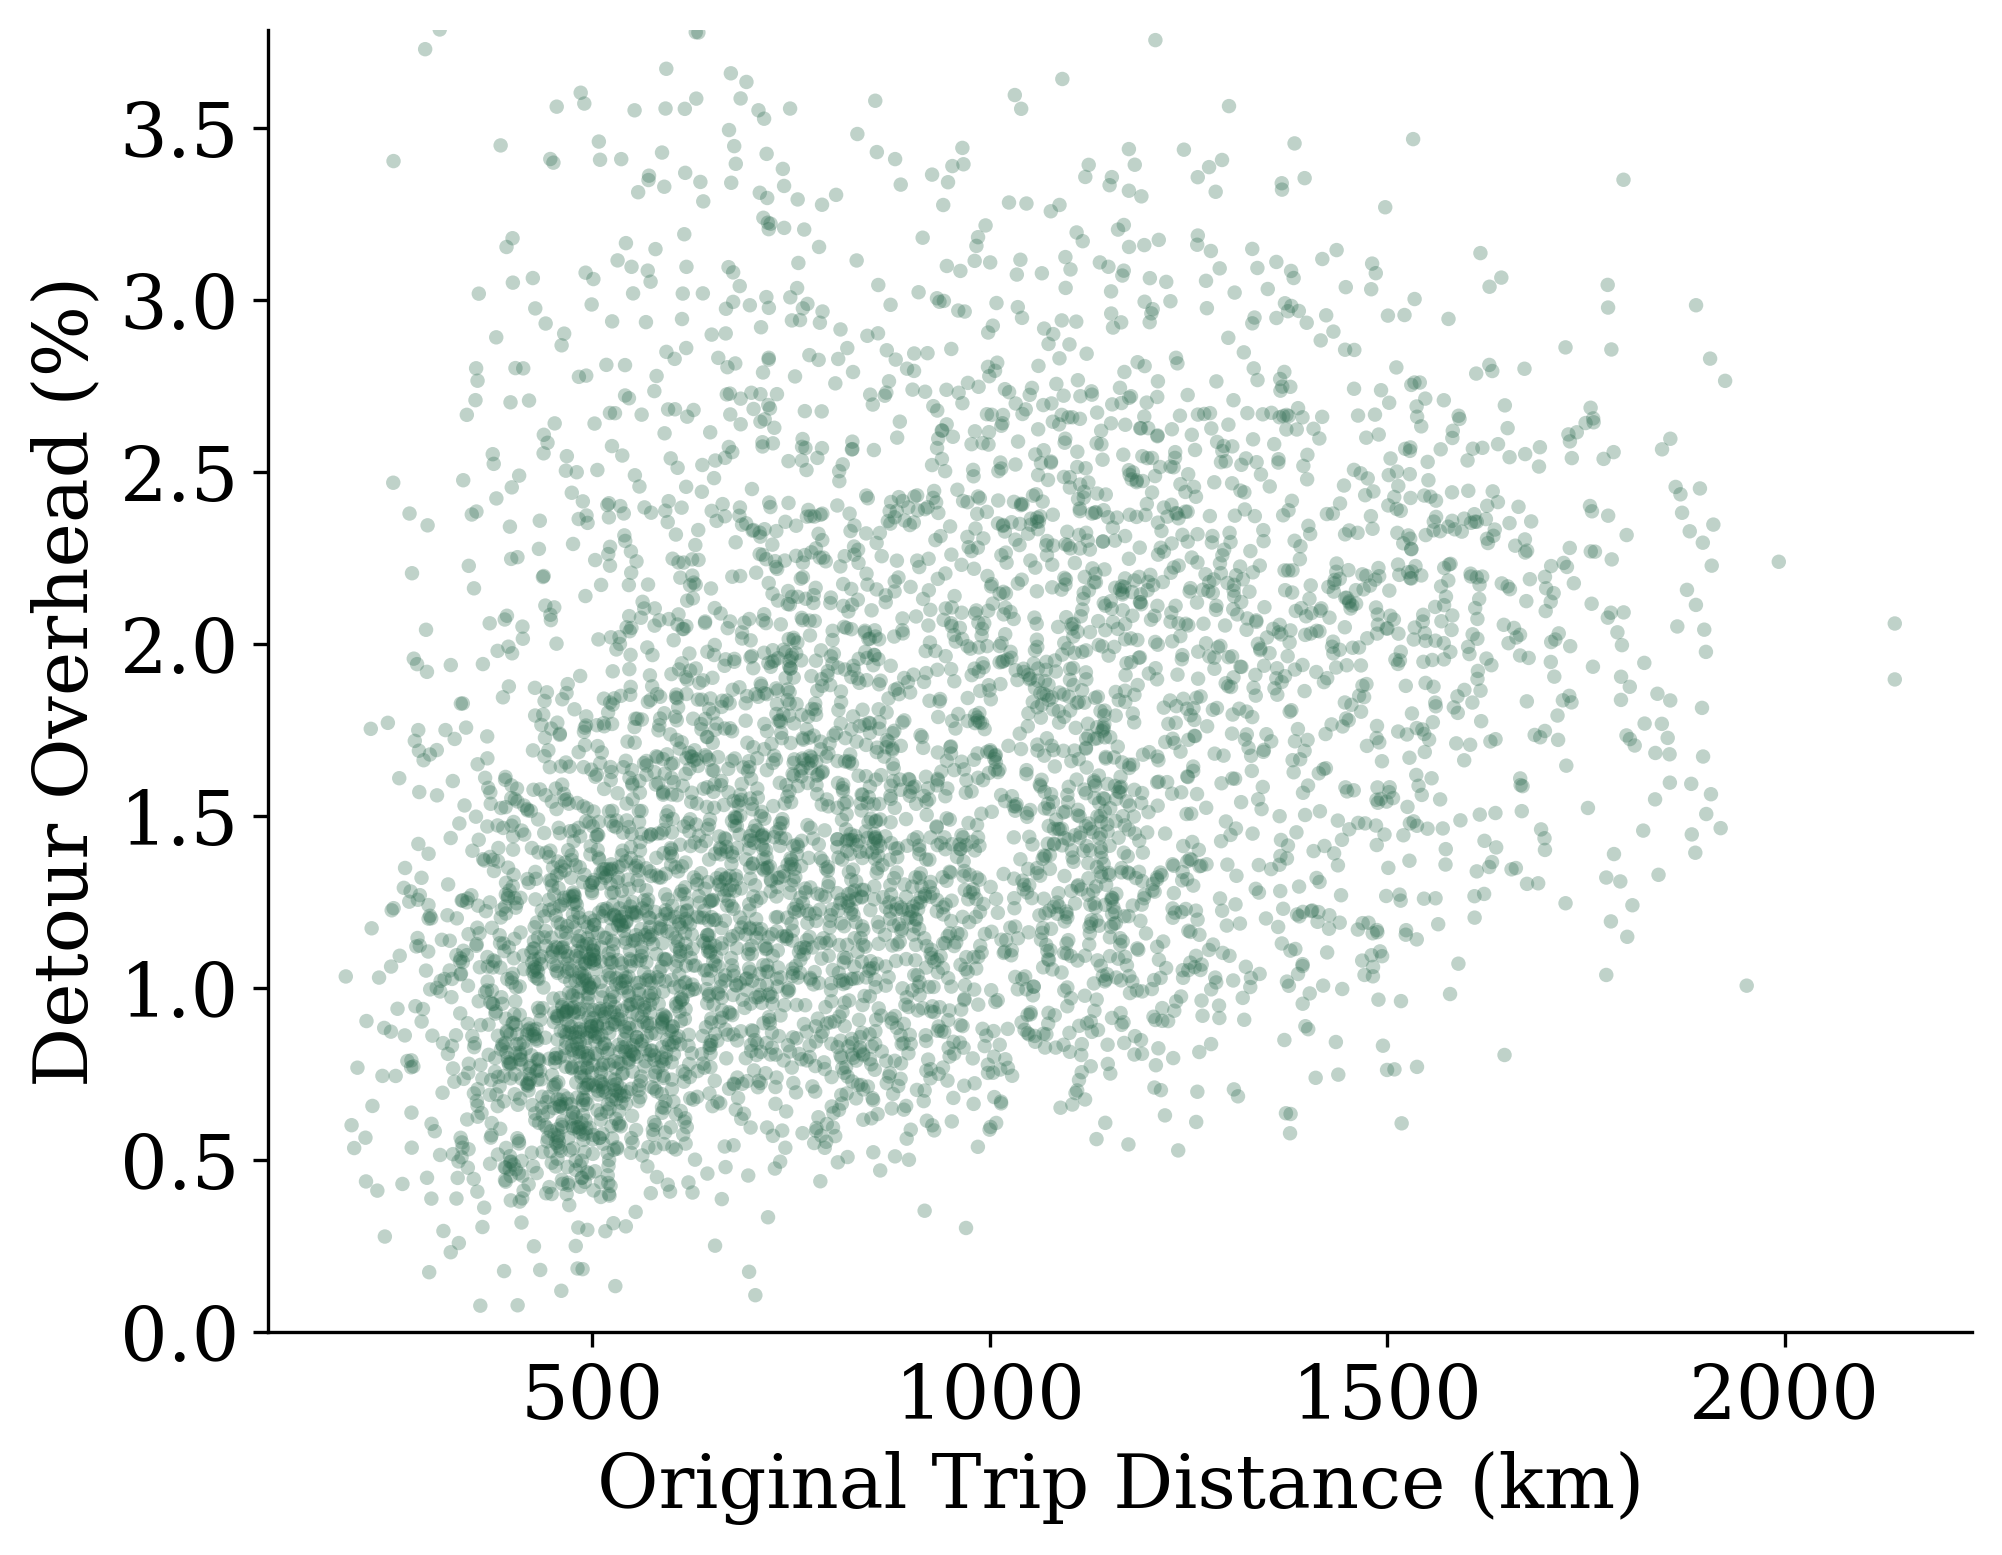
\includegraphics[width=\textwidth]{detour_overhead_350kW_50plugs.png}
    \caption{50 plugs per station}
\end{subfigure}
\hfill
\begin{subfigure}[t]{0.48\textwidth}
    \centering
    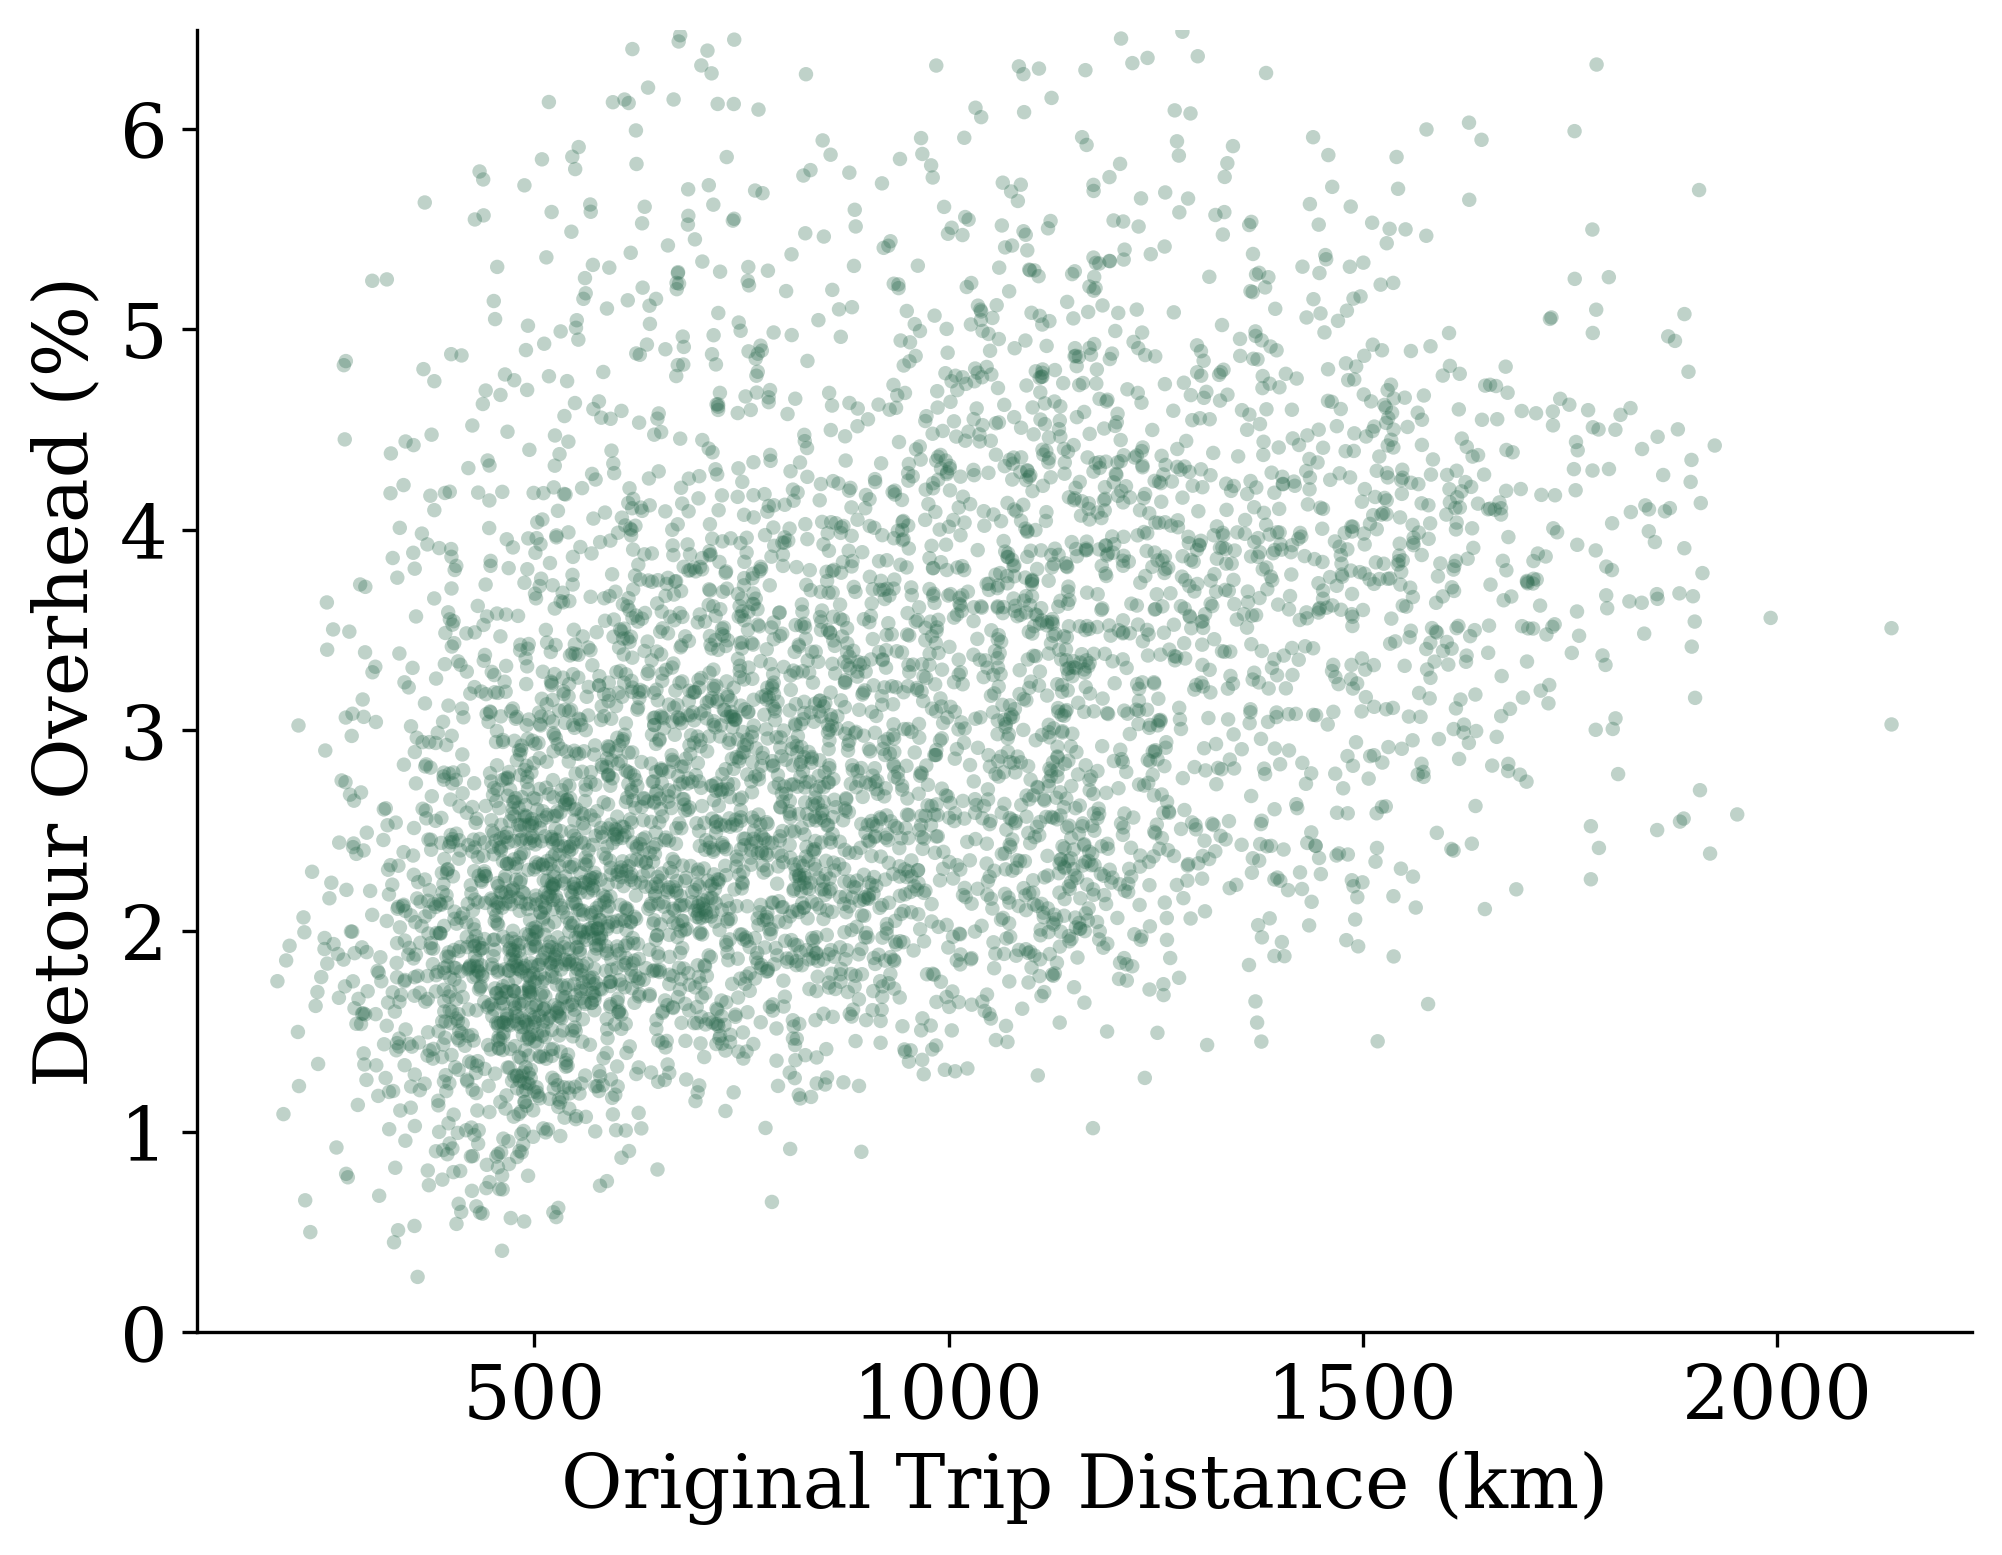
\includegraphics[width=\textwidth]{detour_overhead_350kW_5plugs.png}
    \caption{5 plugs per station}
\end{subfigure}
\caption{Charging detour as a percentage of original trip distance for the 350~kW scenario under two station capacity configurations. Each point represents one feasible path (5,000 randomly sampled for visibility). Reducing station capacity from 50 to 5 plugs nearly doubles the median detour overhead (1.5\% to 2.8\%) as the optimizer routes vehicles to more distant stations.}
\label{fig:detour_overhead}
\end{figure*}

\begin{table*}[!htb]
\centering
\footnotesize
\caption{Case study results: four charger power levels at two plug-count configurations across T\"{u}rkiye's 9,641-station EPDK network. All scenarios achieve 100\% feasibility (2,161,247 feasible paths).}\label{tab:casestudy}
\begin{tabularx}{\textwidth}{l *{4}{>{\centering\arraybackslash}X} | *{4}{>{\centering\arraybackslash}X}}
\toprule
& \multicolumn{4}{c|}{\textbf{50 plugs/station (482,050 total)}} & \multicolumn{4}{c}{\textbf{5 plugs/station (48,205 total)}} \\
\cmidrule(lr){2-5} \cmidrule(lr){6-9}
\textbf{Metric} & \textbf{5 kW} & \textbf{22 kW} & \textbf{50 kW} & \textbf{350 kW} & \textbf{5 kW} & \textbf{22 kW} & \textbf{50 kW} & \textbf{350 kW} \\
\midrule
\multicolumn{9}{l}{\textit{Charging operations}} \\
Avg.\ charge time/stop (min) & 287.3 & 65.0 & 28.6 & 4.1 & 288.1 & 65.6 & 28.8 & 4.1 \\
Avg.\ detour time/path (min) & 17.1 & 13.1 & 11.8 & 9.9 & 23.7 & 22.1 & 21.3 & 18.7 \\
Avg.\ stops/path & 6.1 & 6.1 & 6.1 & 6.1 & 6.2 & 6.1 & 6.1 & 6.1 \\
Additional distance (\%) & 3.0 & 2.3 & 2.0 & 1.7 & 4.1 & 3.8 & 3.7 & 3.2 \\
\midrule
\multicolumn{9}{l}{\textit{Economic analysis (mean savings \%, positive = EV cheaper)}} \\
Tier~1 (Operational) & $+$24.4 & $+$25.0 & $+$25.2 & $+$25.5 & $+$23.2 & $+$23.5 & $+$23.6 & $+$24.1 \\
Tier~2 (TCO) & $+$10.9 & $+$11.3 & $+$11.5 & $+$11.7 & $+$10.0 & $+$10.3 & $+$10.4 & $+$10.7 \\
Tier~3 (Infrastructure) & $-$15.8 & $-$15.4 & $-$15.2 & $-$15.0 & $+$7.4 & $+$7.6 & $+$7.7 & $+$8.0 \\
\midrule
\multicolumn{9}{l}{\textit{Paths with EV cheaper (\%)}} \\
Tier~1 & 100.0 & 100.0 & 100.0 & 100.0 & 100.0 & 100.0 & 100.0 & 100.0 \\
Tier~2 & 96.7 & 97.0 & 97.1 & 97.2 & 96.0 & 96.2 & 96.3 & 96.6 \\
\bottomrule
\end{tabularx}
\end{table*}



\subsection{Sensitivity Analysis}\label{sec:sensitivity}

To identify which EV technology and operational parameters most influence the viability of intercity electric travel in T\"{u}rkiye, four univariate parameter sweeps are conducted. Each sweep varies one parameter across five levels while holding all others at their baseline values (\cref{tab:params}). A 1\% electrification rate is applied, randomly sampling 1\% of vehicles from the pre-computed trajectory set, with 10 replications per parameter level using distinct random seeds to capture stochastic variability. The four parameters and their levels are: EV range ($\underline{R}$--$\overline{R}$, km) at (150, 250), (250, 400), (400, 550), (550, 700), and (700, 900); discharge rate upper bound ($\overline{\rho}$, Wh/km) at 150, 160, 190, 220, and 250; charger power ($W_c$, kW) at 50, 100, 250, 350, and 500; and operational SoC bounds ($\underline{S}$--$\overline{S}$, \%) at (5, 100), (10, 100), (10, 80), (20, 100), and (20, 80). Each sweep comprises 5 levels $\times$ 10 replications = 50 runs, yielding 200 individual runs in total.

The sensitivity analysis focuses on Tier~1 and Tier~2 outcomes. Tier~3 (Infrastructure) is excluded from the sensitivity sweeps because the per-trip infrastructure amortization term in \eqref{eq:t3ev} depends on the total plug count and estimated national vehicle count, which are fixed inputs unaffected by the four swept parameters. Tier~3 results are reported in \cref{sec:casestudy}, where charger power and plug count vary across scenarios.

The discharge rate upper bound produces the largest economic sensitivity. Its Tier~2 span is 12.5 percentage points, ranging from $+12.5$\% at 250~Wh/km (baseline) to $+25.0$\% at 150~Wh/km, and its Tier~1 span reaches 18.3 percentage points (\cref{fig:sensitivity_summary,fig:sensitivity_tier2}). Lower discharge rates reduce electricity consumption per kilometer, directly cutting energy costs without altering feasibility, which remains at 100\% across all levels. This effect is amplified in T\"{u}rkiye by the high public charger electricity price (13~TL/kWh), making energy efficiency the most impactful lever for improving intercity EV cost competitiveness. The charging operations metrics (\cref{fig:sensitivity_ops}) confirm that discharge rate has no effect on the number of stops, detour time, or additional distance, reinforcing that its impact is purely economic rather than operational.

EV range produces the second-largest Tier~2 span at 5.9 percentage points, from $+10.2$\% (150--250~km) to $+16.1$\% (700--900~km). Under the baseline SoC operating window of 10--100\%, all range levels achieve 100\% feasibility, meaning that even short-range EVs can complete intercity trips through more frequent charging stops. The Tier~1 operational savings are nearly flat ($+26.2$\% to $+26.7$\%), indicating that range primarily affects the per-trip vehicle cost component through TCO amortization rather than energy or time consumption. Short-range vehicles require slightly more stops (7.6 vs.\ 6.0) and longer detours (5.6 vs.\ 3.4~min), but these operational differences are modest (\cref{fig:sensitivity_ops}).

The operational SoC bounds parameter reveals the most dramatic structural effect. When $\overline{S} = 100$\%, feasibility remains at 100\% regardless of the lower bound; when $\overline{S}$ is capped at 80\%, feasibility collapses to just 0.3\%. This cliff occurs because T\"{u}rkiye's highway network contains stretches between consecutive charger opportunities whose cumulative energy consumption exceeds the usable SoC window under the 80\% cap but falls within the wider window when $\overline{S} = 100$\%. The Tier~2 range across SoC bound levels is modest (2.0~pp) because the metric is computed only over feasible paths, which are nearly identical in the three wide-window scenarios and negligible in the two narrow-window scenarios. The practical implication is that T\"{u}rkiye's current charging network can support intercity EV travel for vehicles that utilize their full battery capacity but is inadequate for vehicles constrained to a conventional 20--80\% operating range, highlighting the need either for denser charger deployment in underserved corridors or for battery management systems that safely extend the usable SoC window.

Charger power produces essentially zero Tier~2 sensitivity (0.0~pp), with savings stable at $+12.5$\% across all power levels from 50 to 500~kW. Charging time per stop varies substantially, from 27.6~min at 50~kW to 2.8~min at 500~kW (\cref{fig:sensitivity_ops}), but at a 1\% electrification rate congestion is nonexistent and charging duration does not translate into queue-based wait costs. Charger power is therefore a capacity parameter whose importance scales with the EV adoption rate rather than an efficiency parameter affecting individual trip economics.

\begin{figure}[!ht]
\centering
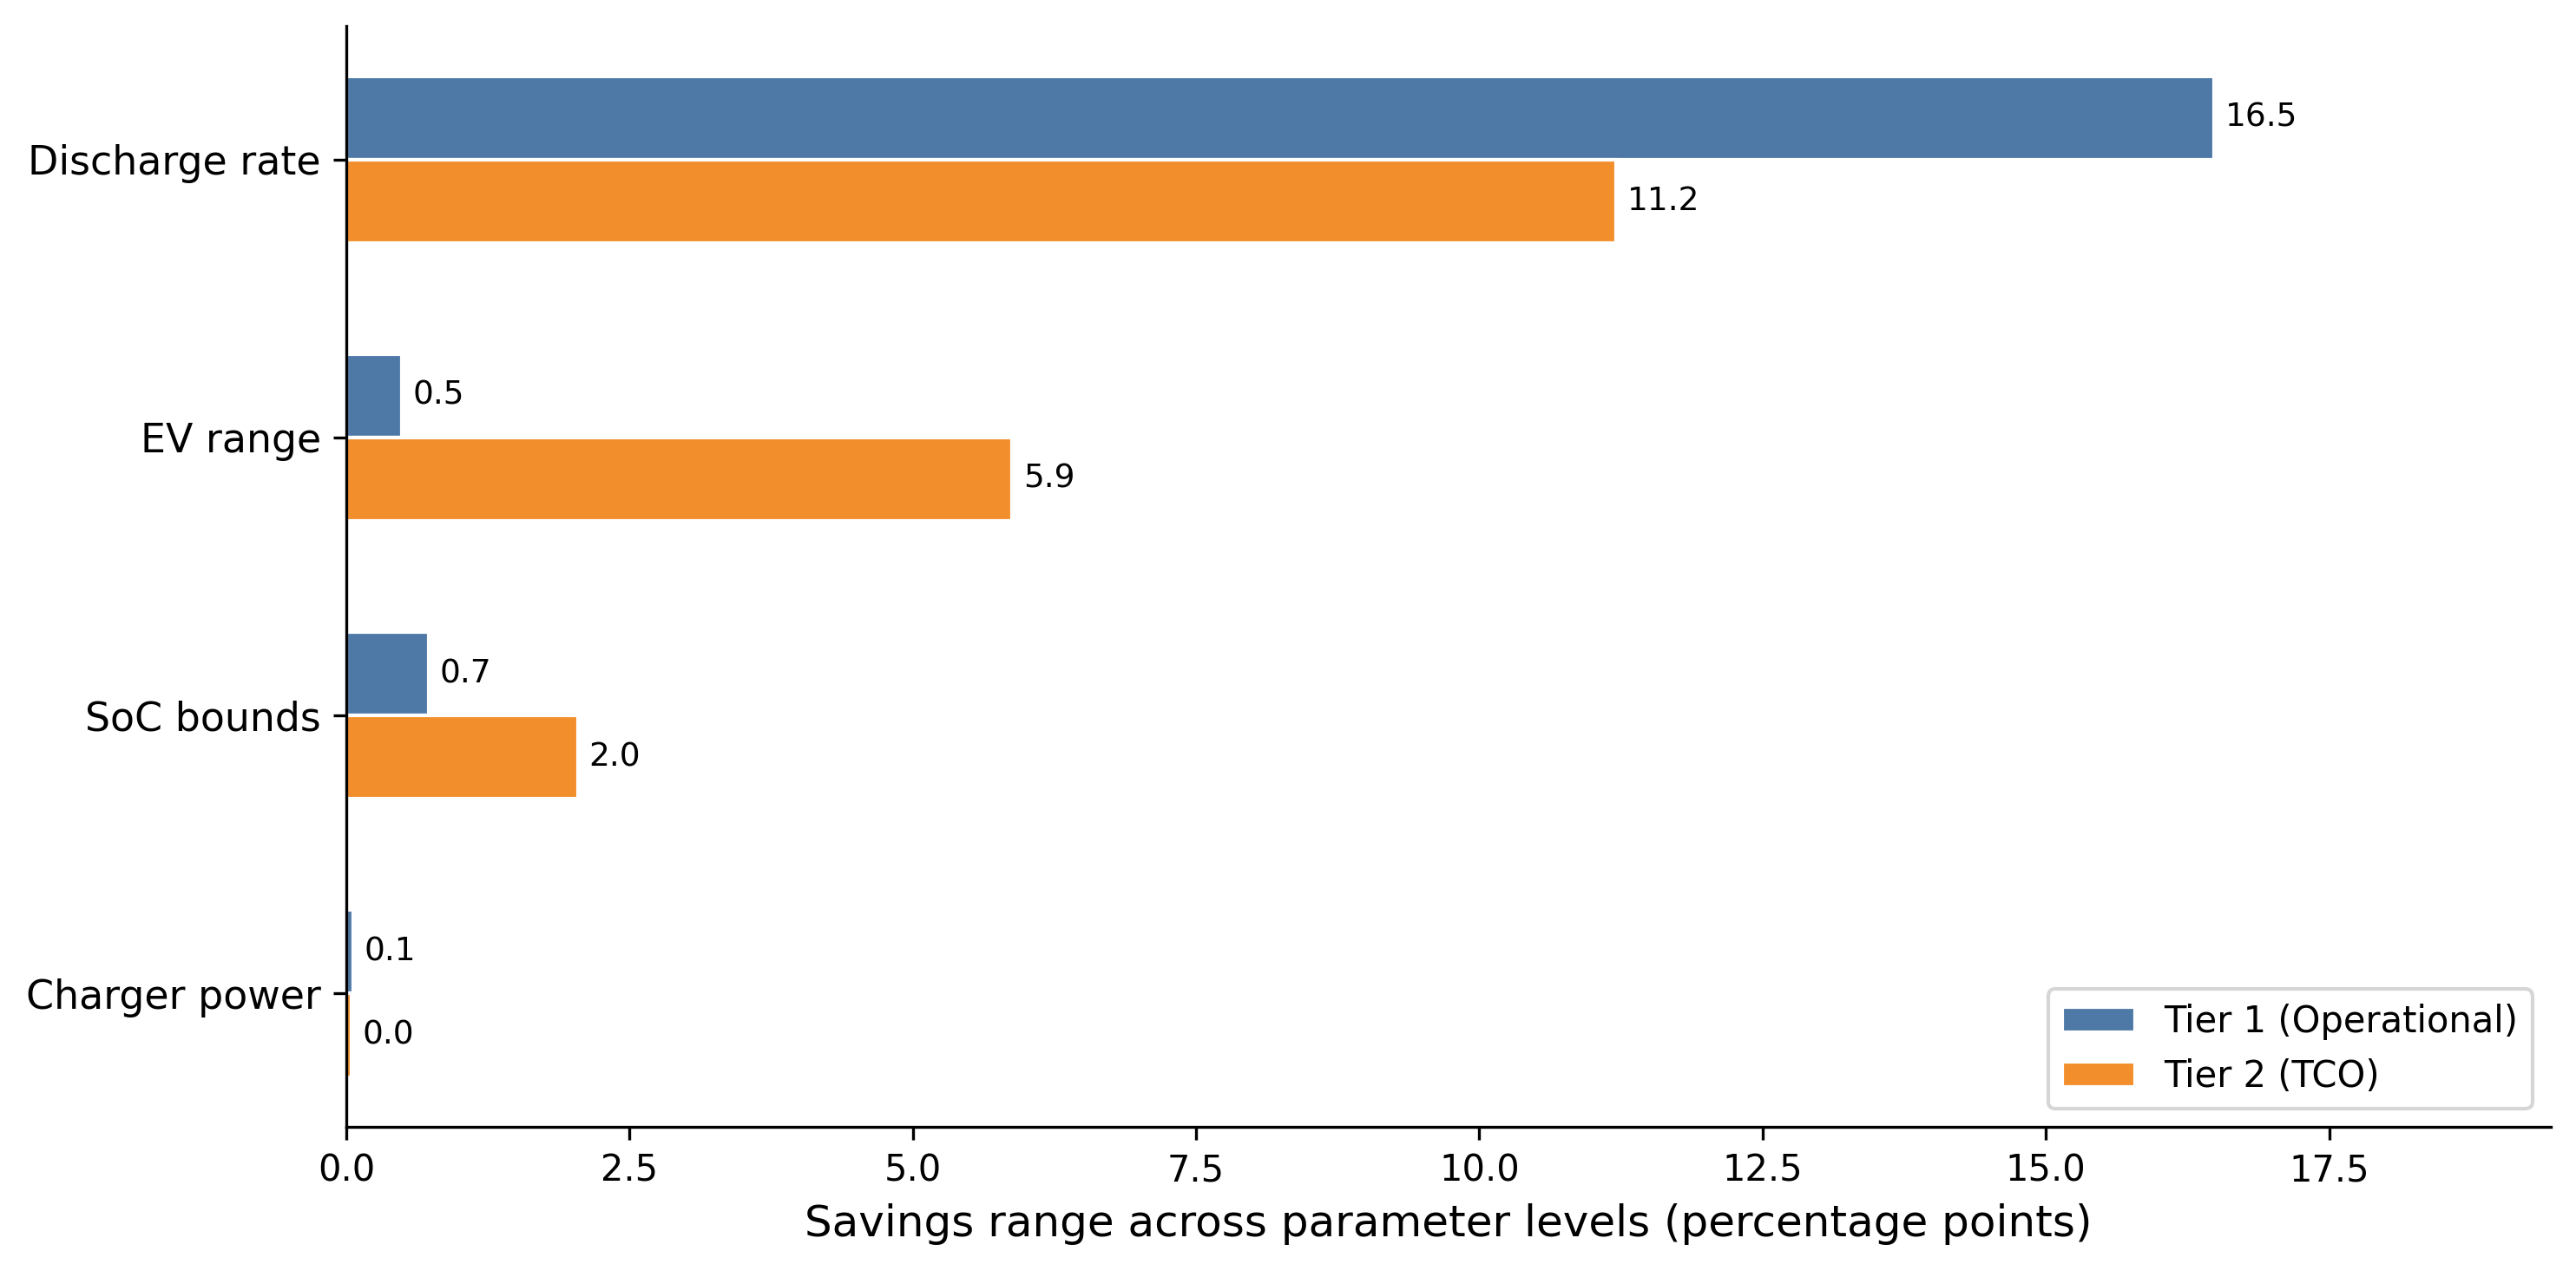
\includegraphics[width=0.85\linewidth]{sensitivity_summary_tr.png}
\caption{Sensitivity range (in percentage points) of mean savings across parameter levels for Tier~1 (Operational) and Tier~2 (TCO).}
\label{fig:sensitivity_summary}
\end{figure}

\begin{figure*}[!htb]
\centering
\begin{subfigure}[t]{0.48\textwidth}
    \centering
    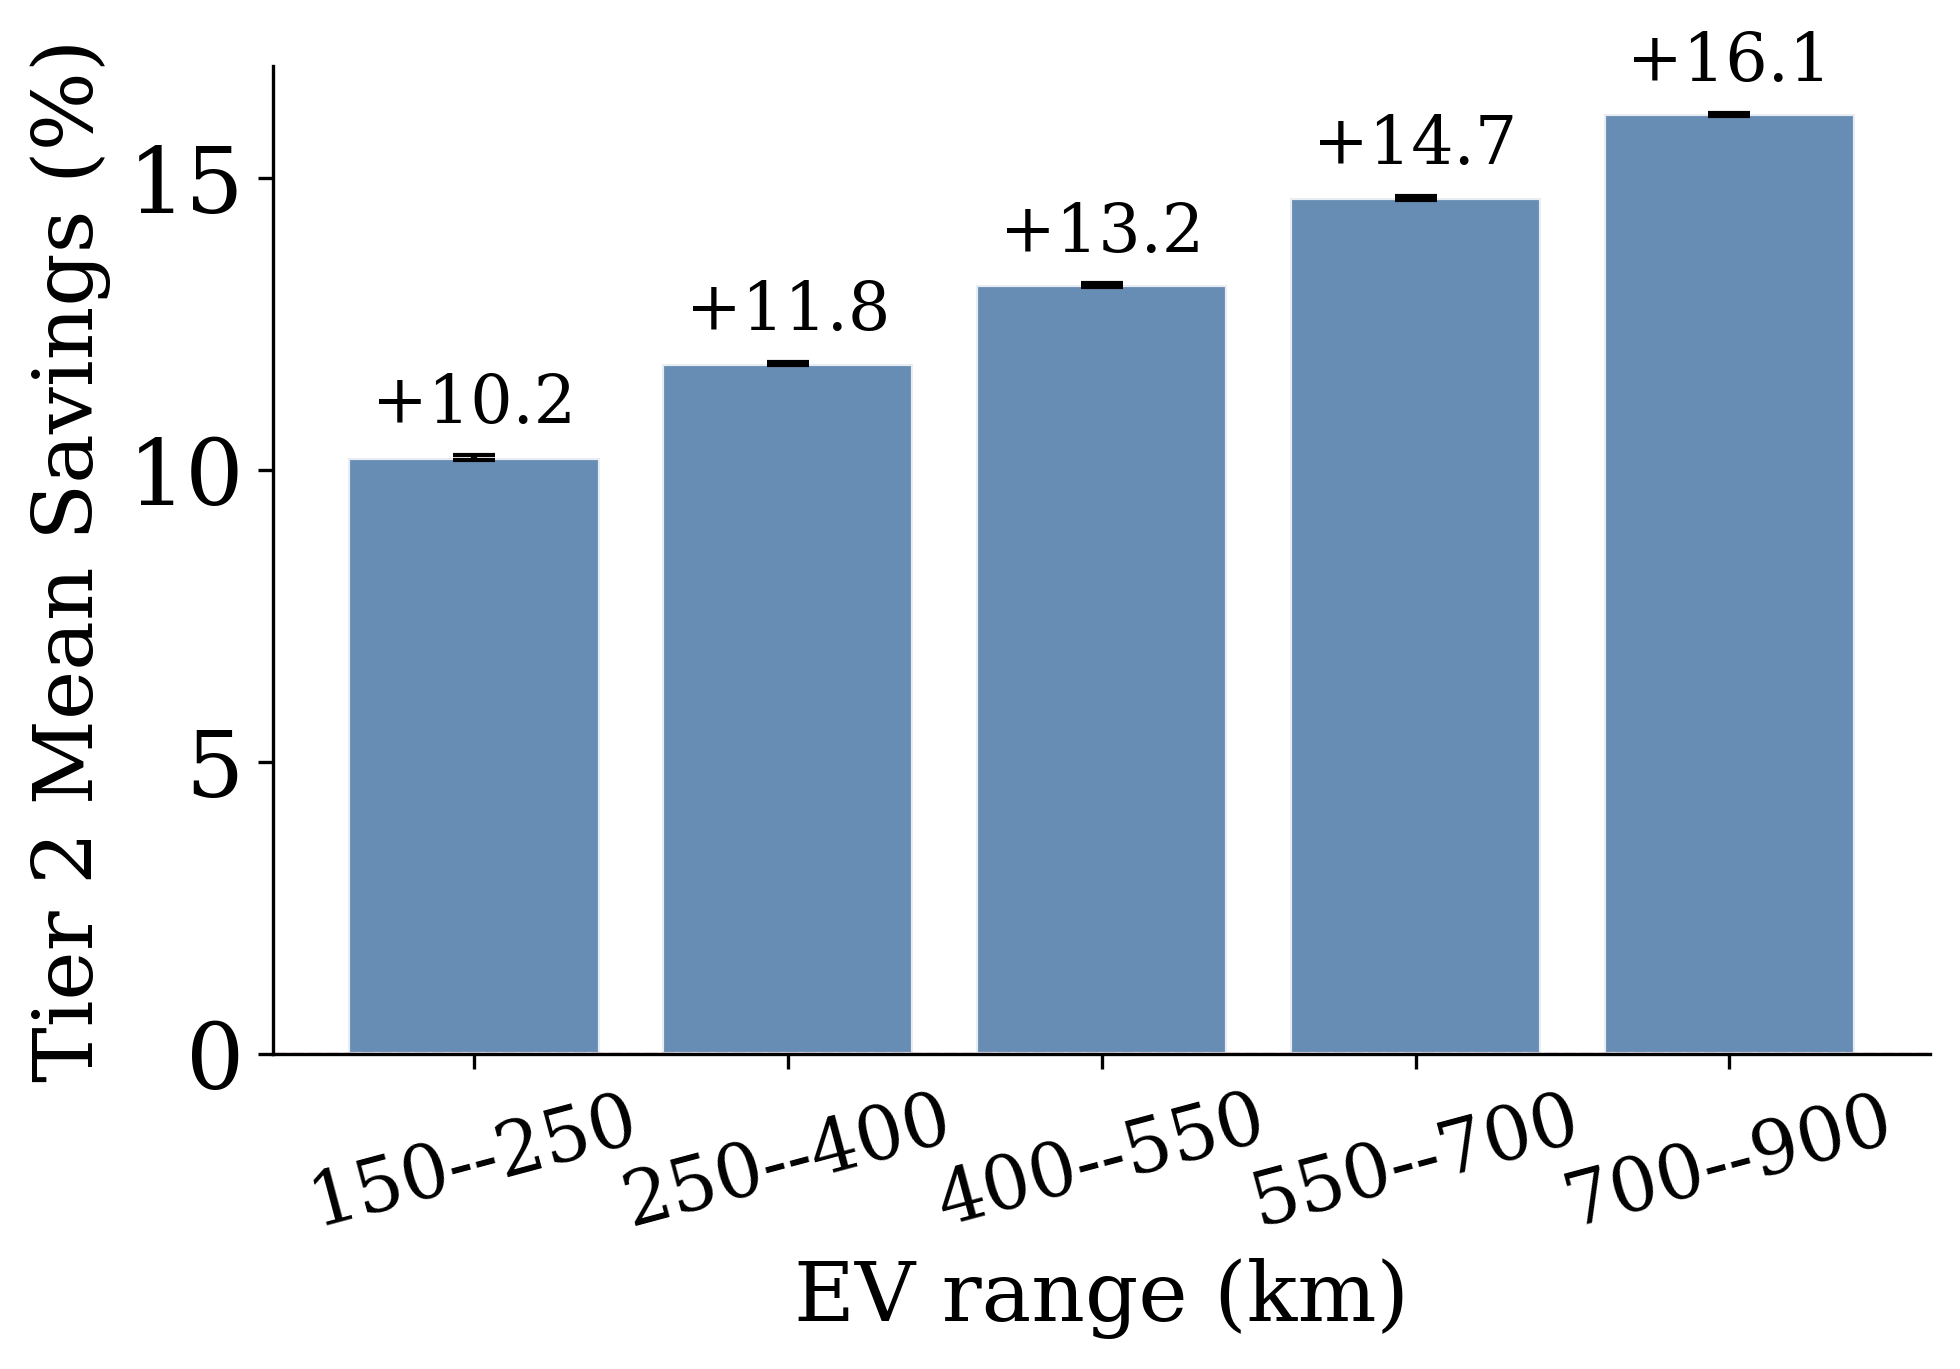
\includegraphics[width=\textwidth]{sensitivity_tier2_range_tr.png}
    \caption{EV range}
\end{subfigure}
\hfill
\begin{subfigure}[t]{0.48\textwidth}
    \centering
    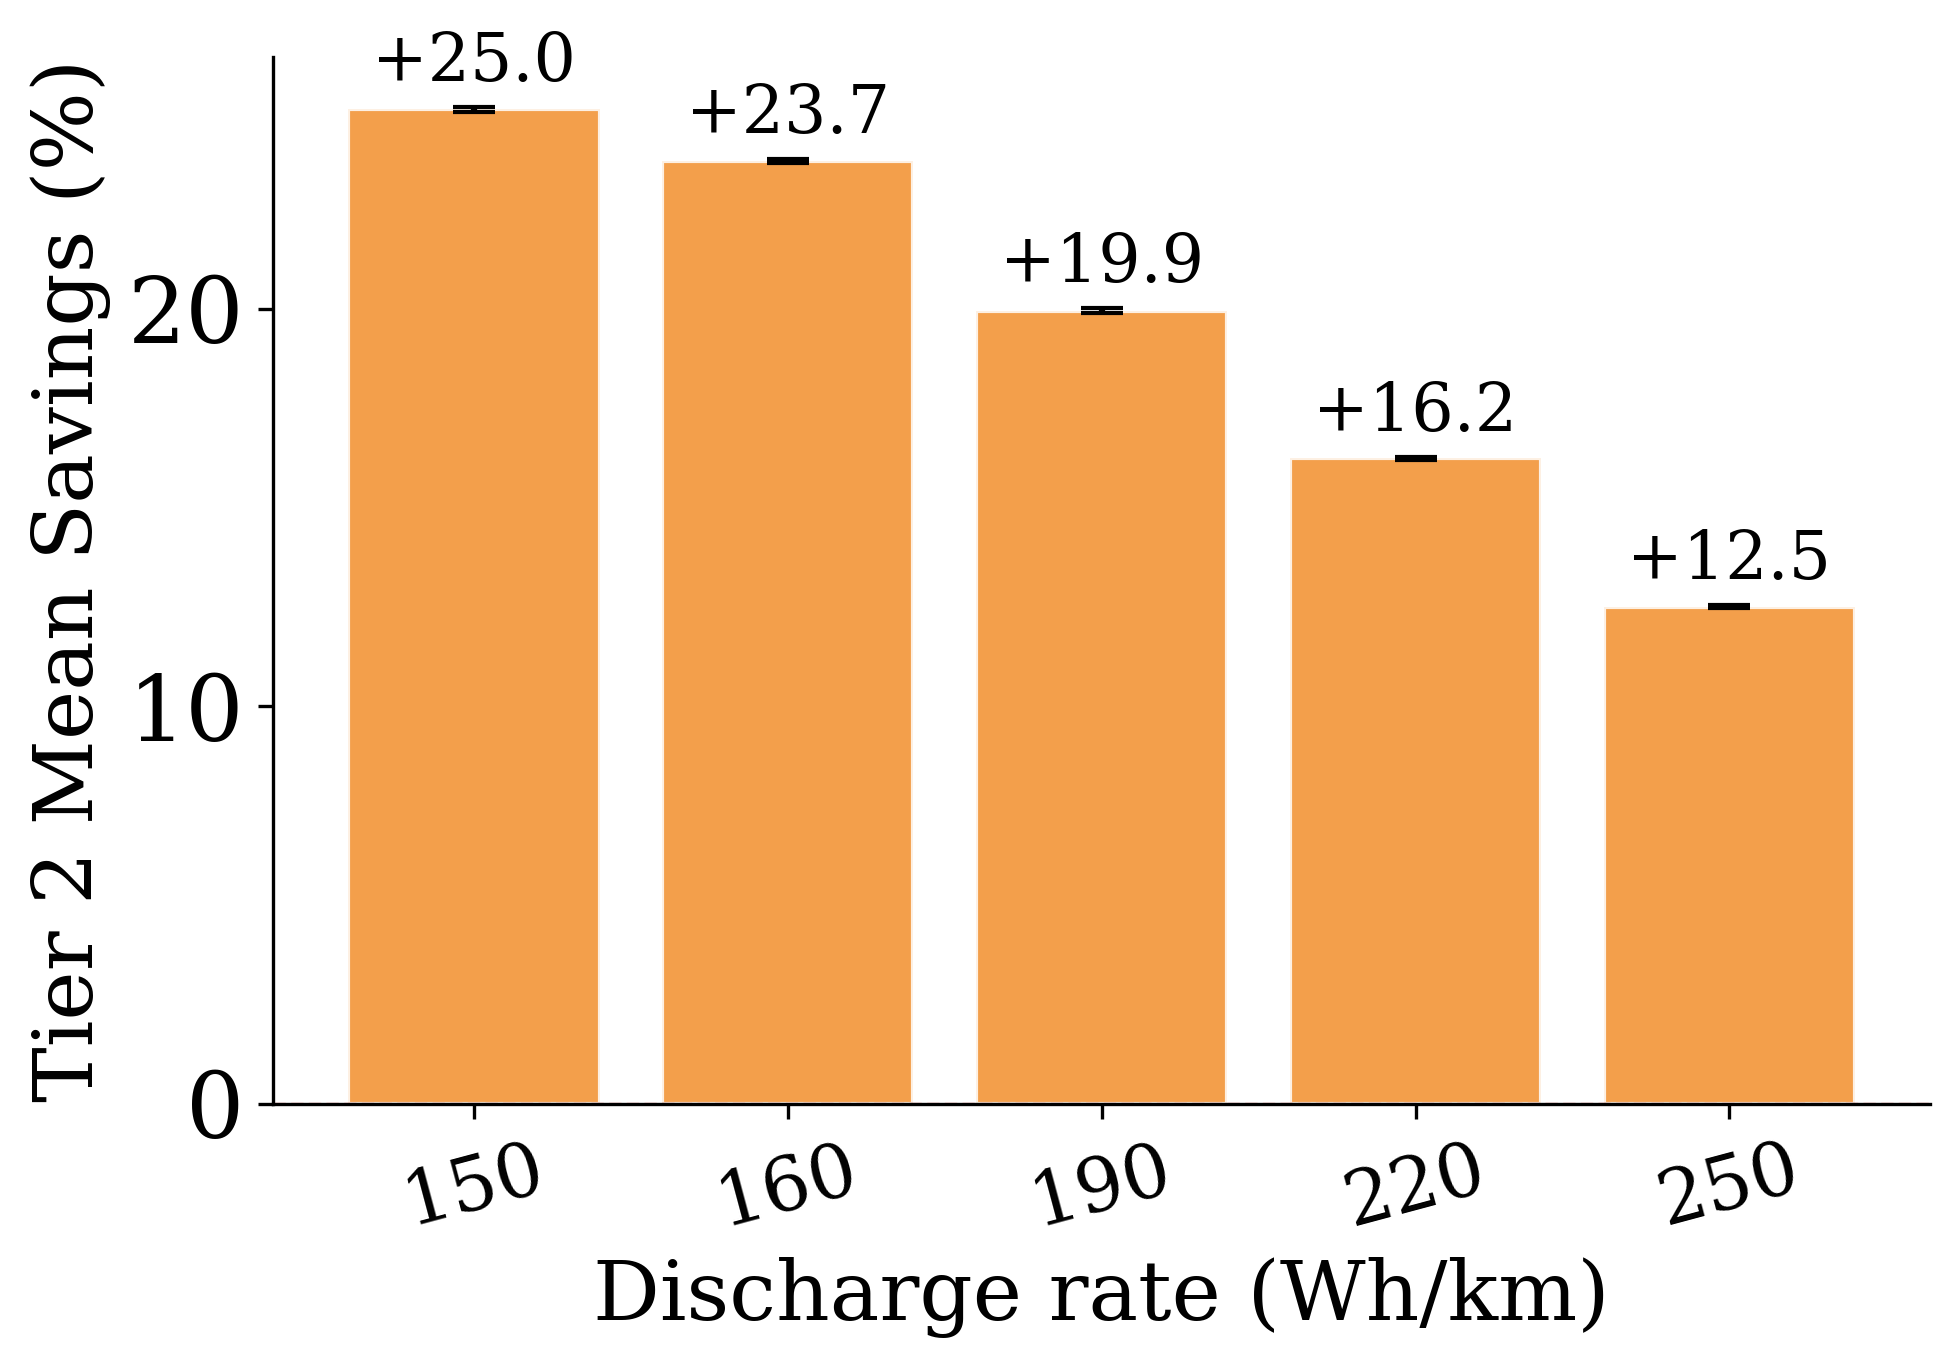
\includegraphics[width=\textwidth]{sensitivity_tier2_discharge_tr.png}
    \caption{Discharge rate}
\end{subfigure}

\vspace{6pt}
\begin{subfigure}[t]{0.48\textwidth}
    \centering
    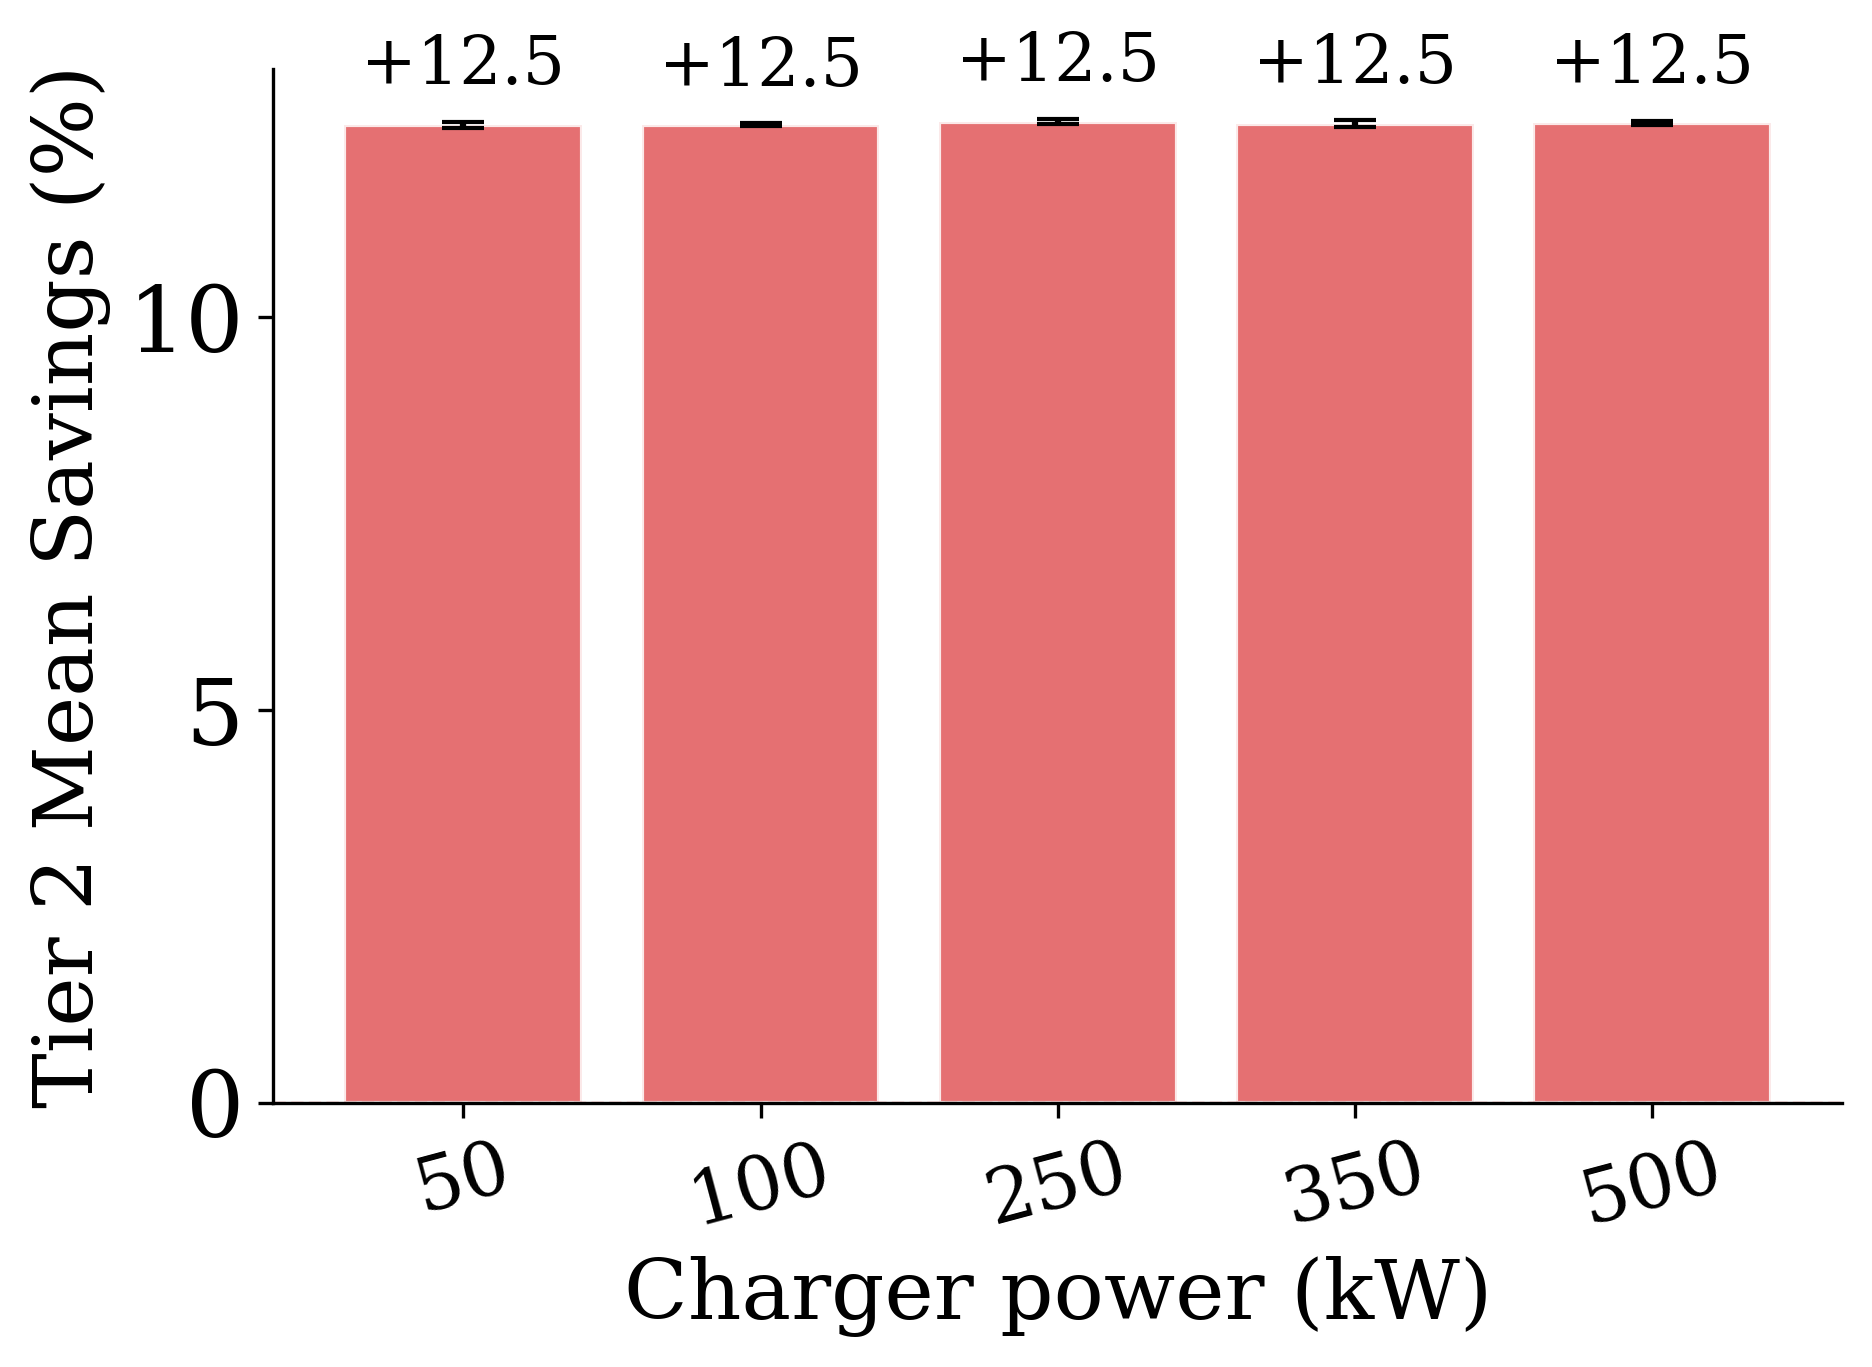
\includegraphics[width=\textwidth]{sensitivity_tier2_power_tr.png}
    \caption{Charger power}
\end{subfigure}
\hfill
\begin{subfigure}[t]{0.48\textwidth}
    \centering
    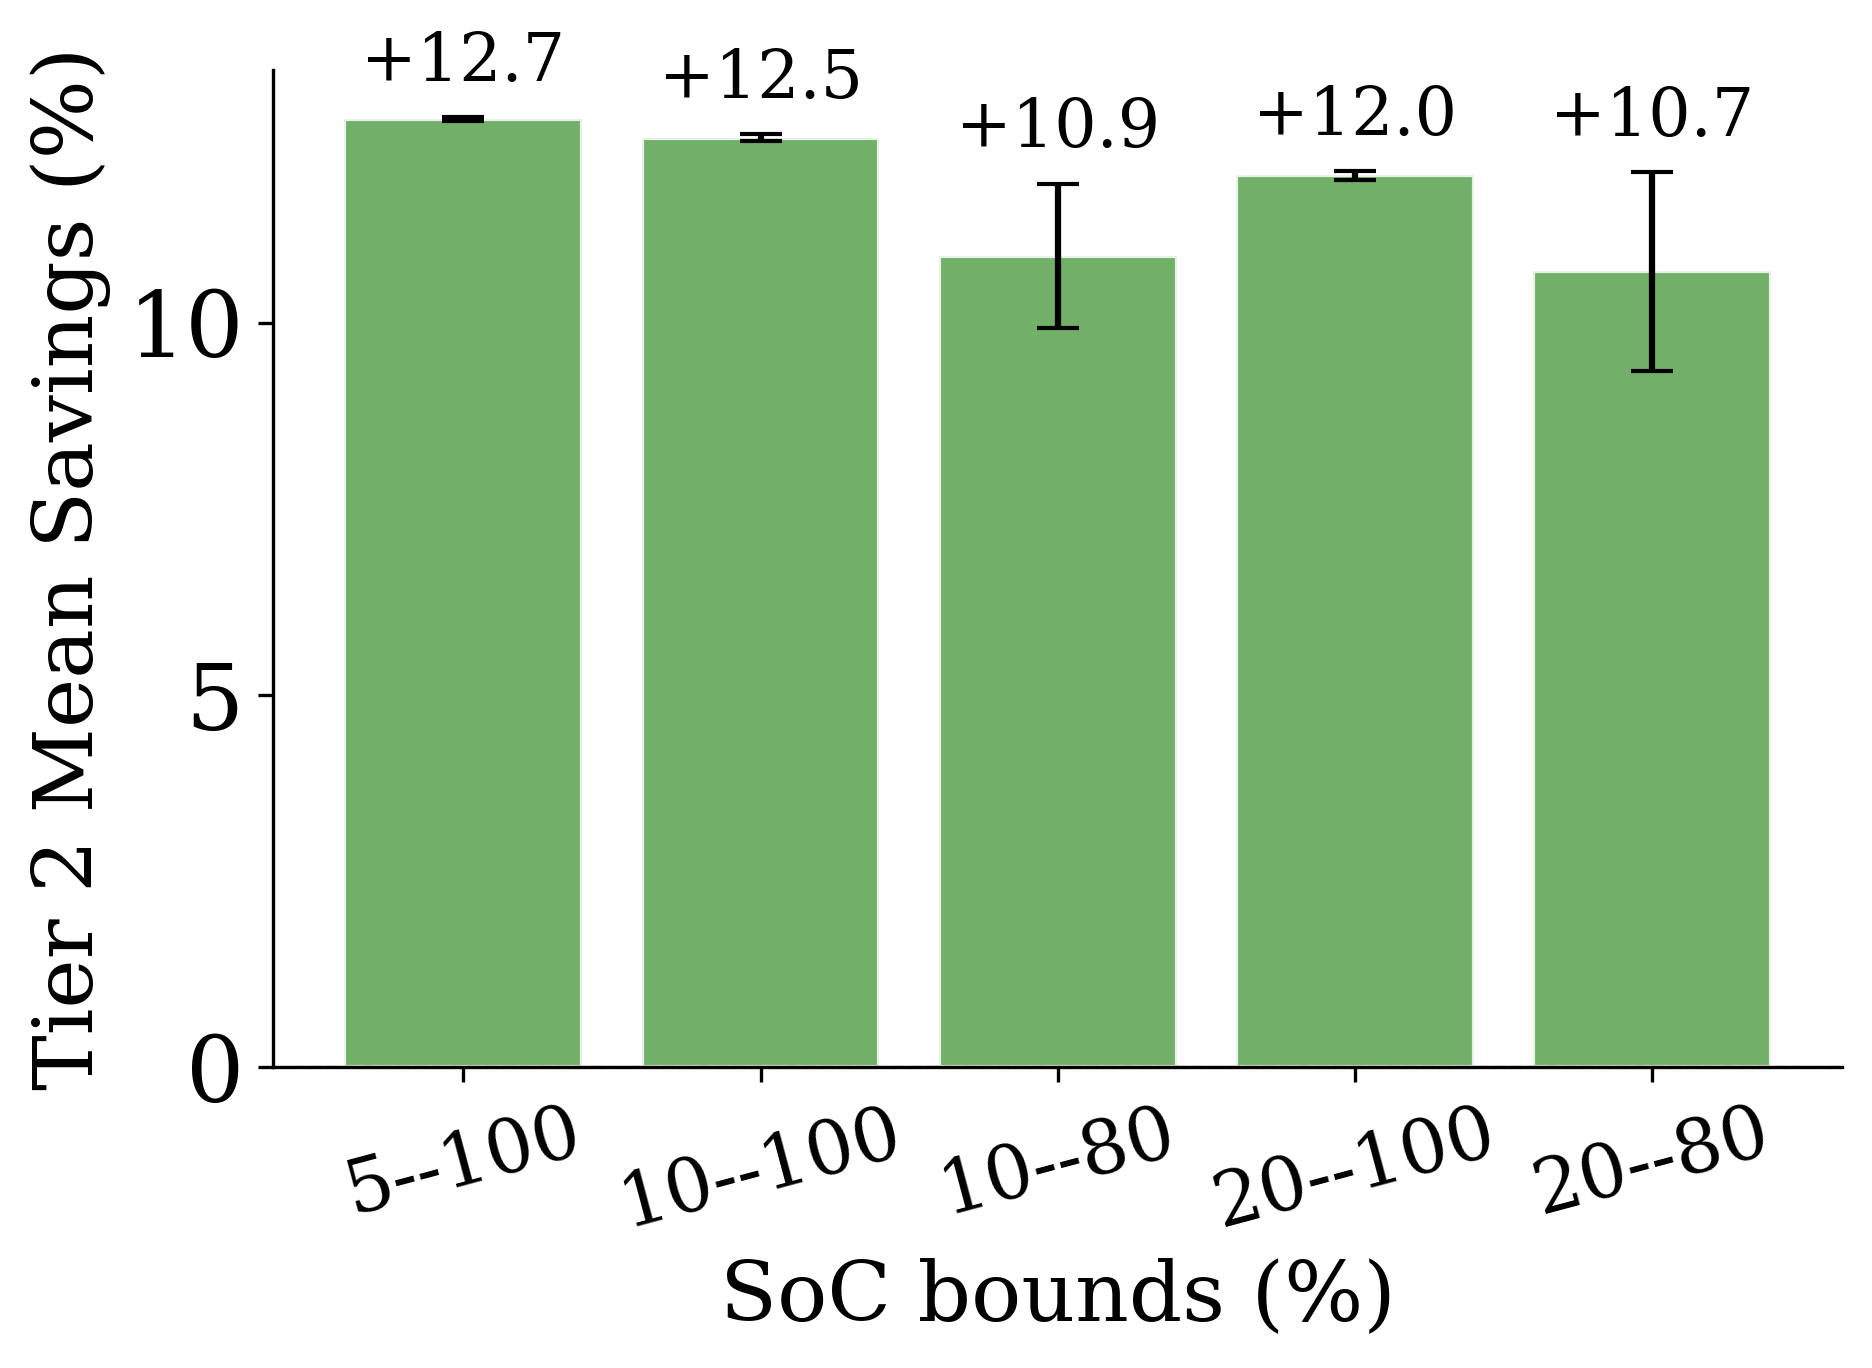
\includegraphics[width=\textwidth]{sensitivity_tier2_soc_tr.png}
    \caption{SoC bounds}
\end{subfigure}
\caption{Tier~2 (TCO) mean savings by parameter level across the four sensitivity sweeps. Error bars show $\pm$1 standard deviation over 10 replications.}
\label{fig:sensitivity_tier2}
\end{figure*}

\begin{figure*}[!htb]
\centering
\begin{subfigure}[t]{0.48\textwidth}
    \centering
    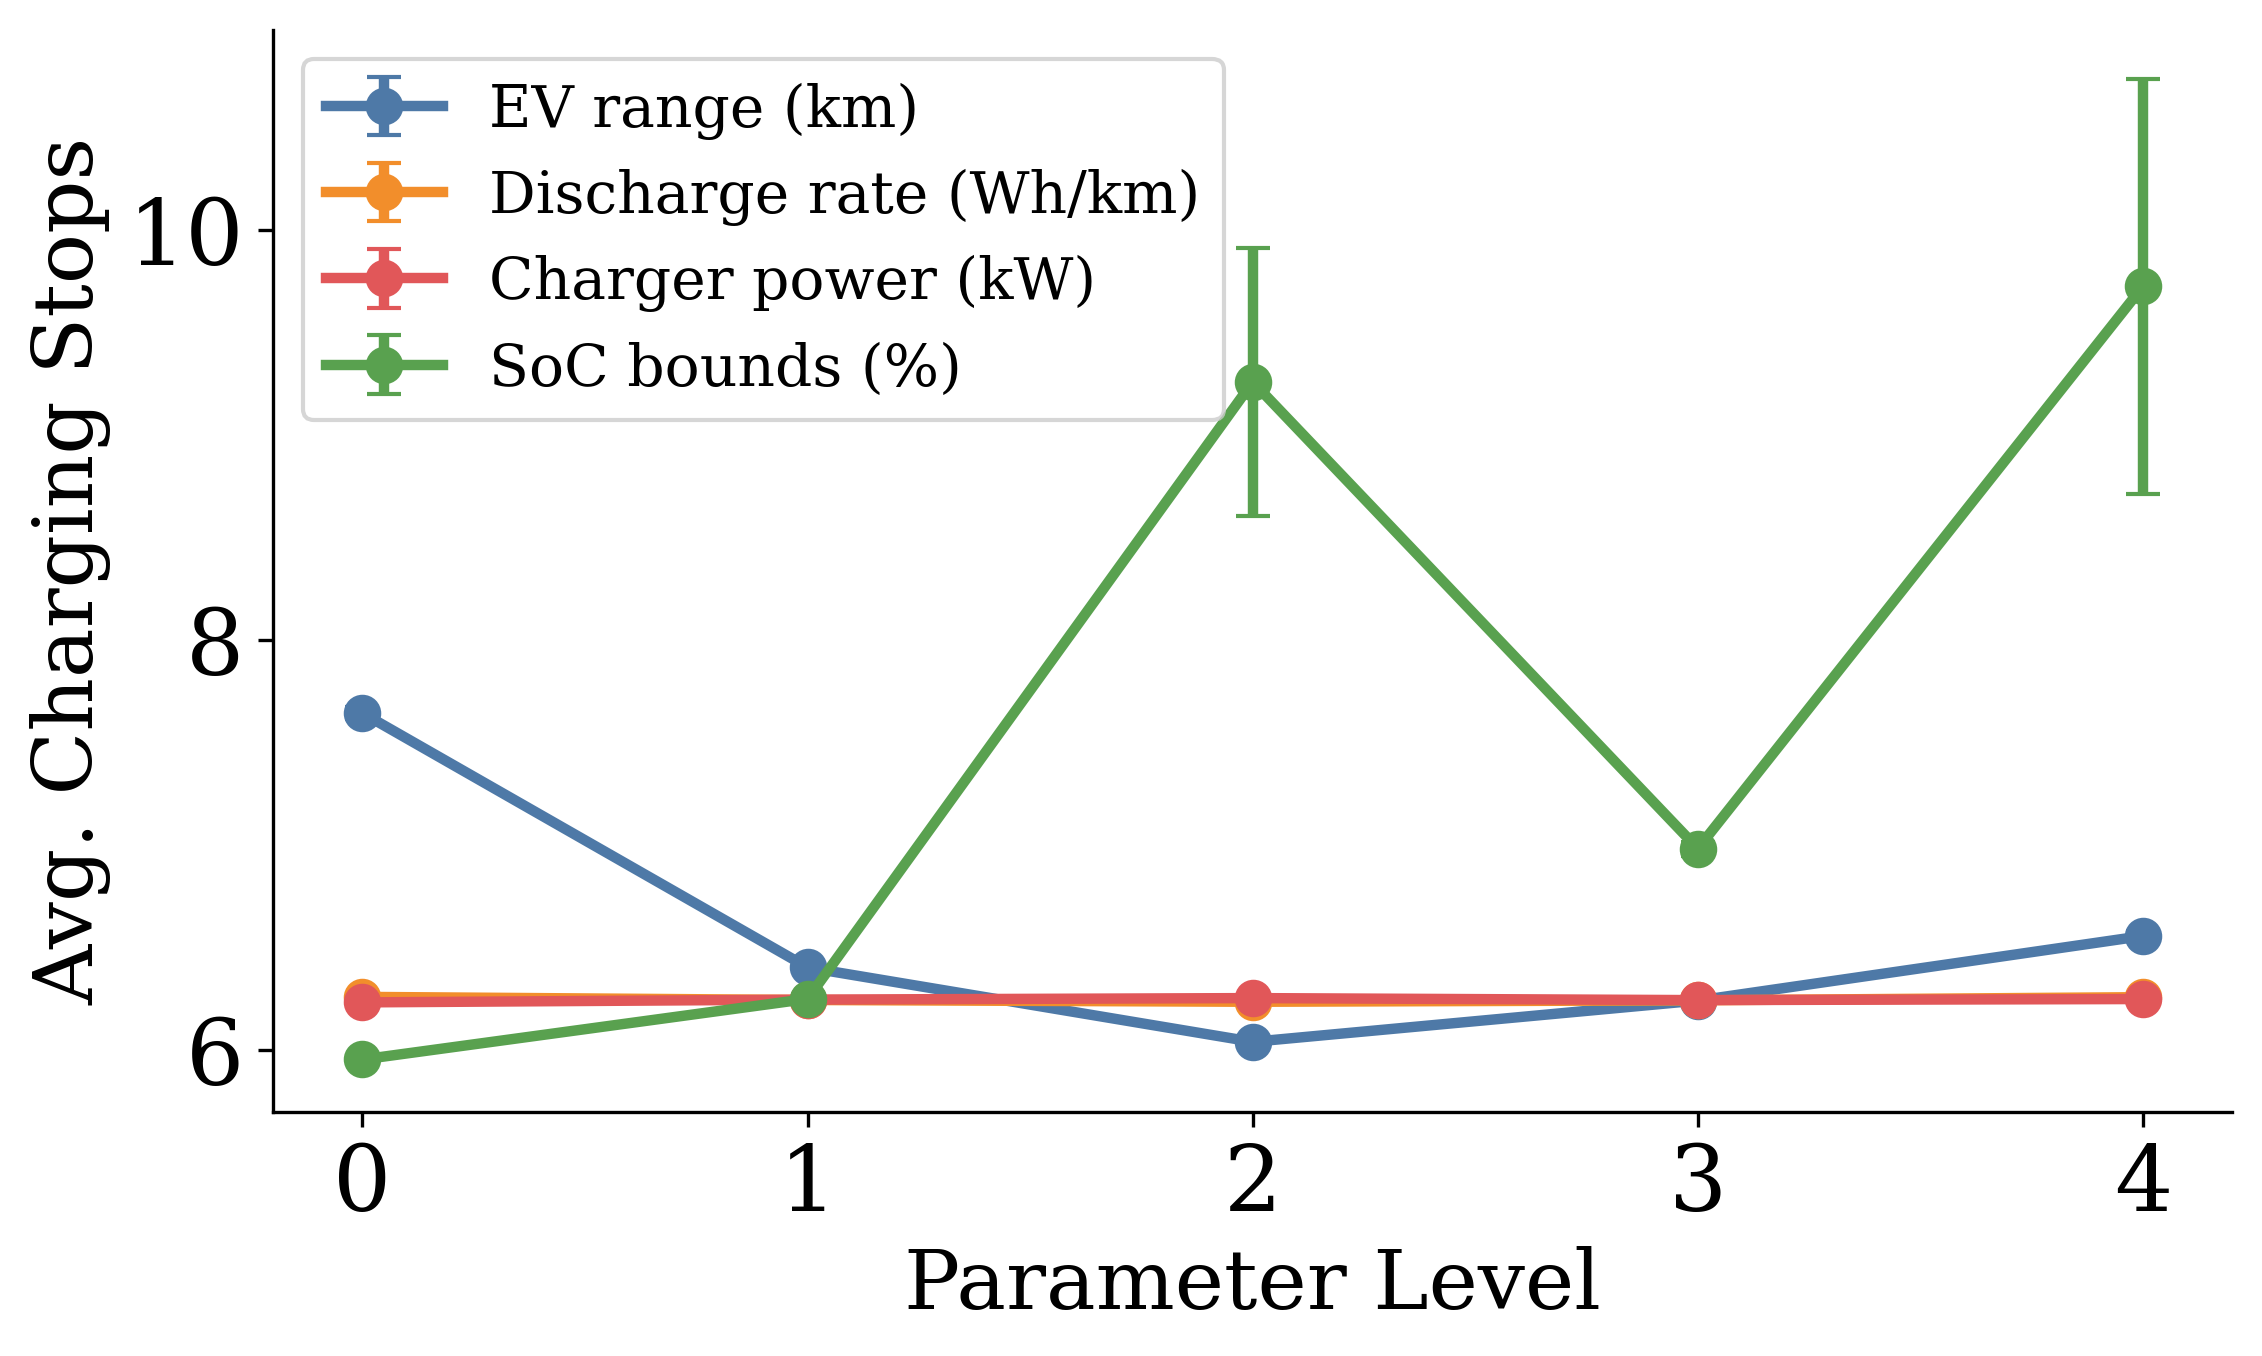
\includegraphics[width=\textwidth]{sensitivity_stops_tr.png}
    \caption{Average charging stops per path}
\end{subfigure}
\hfill
\begin{subfigure}[t]{0.48\textwidth}
    \centering
    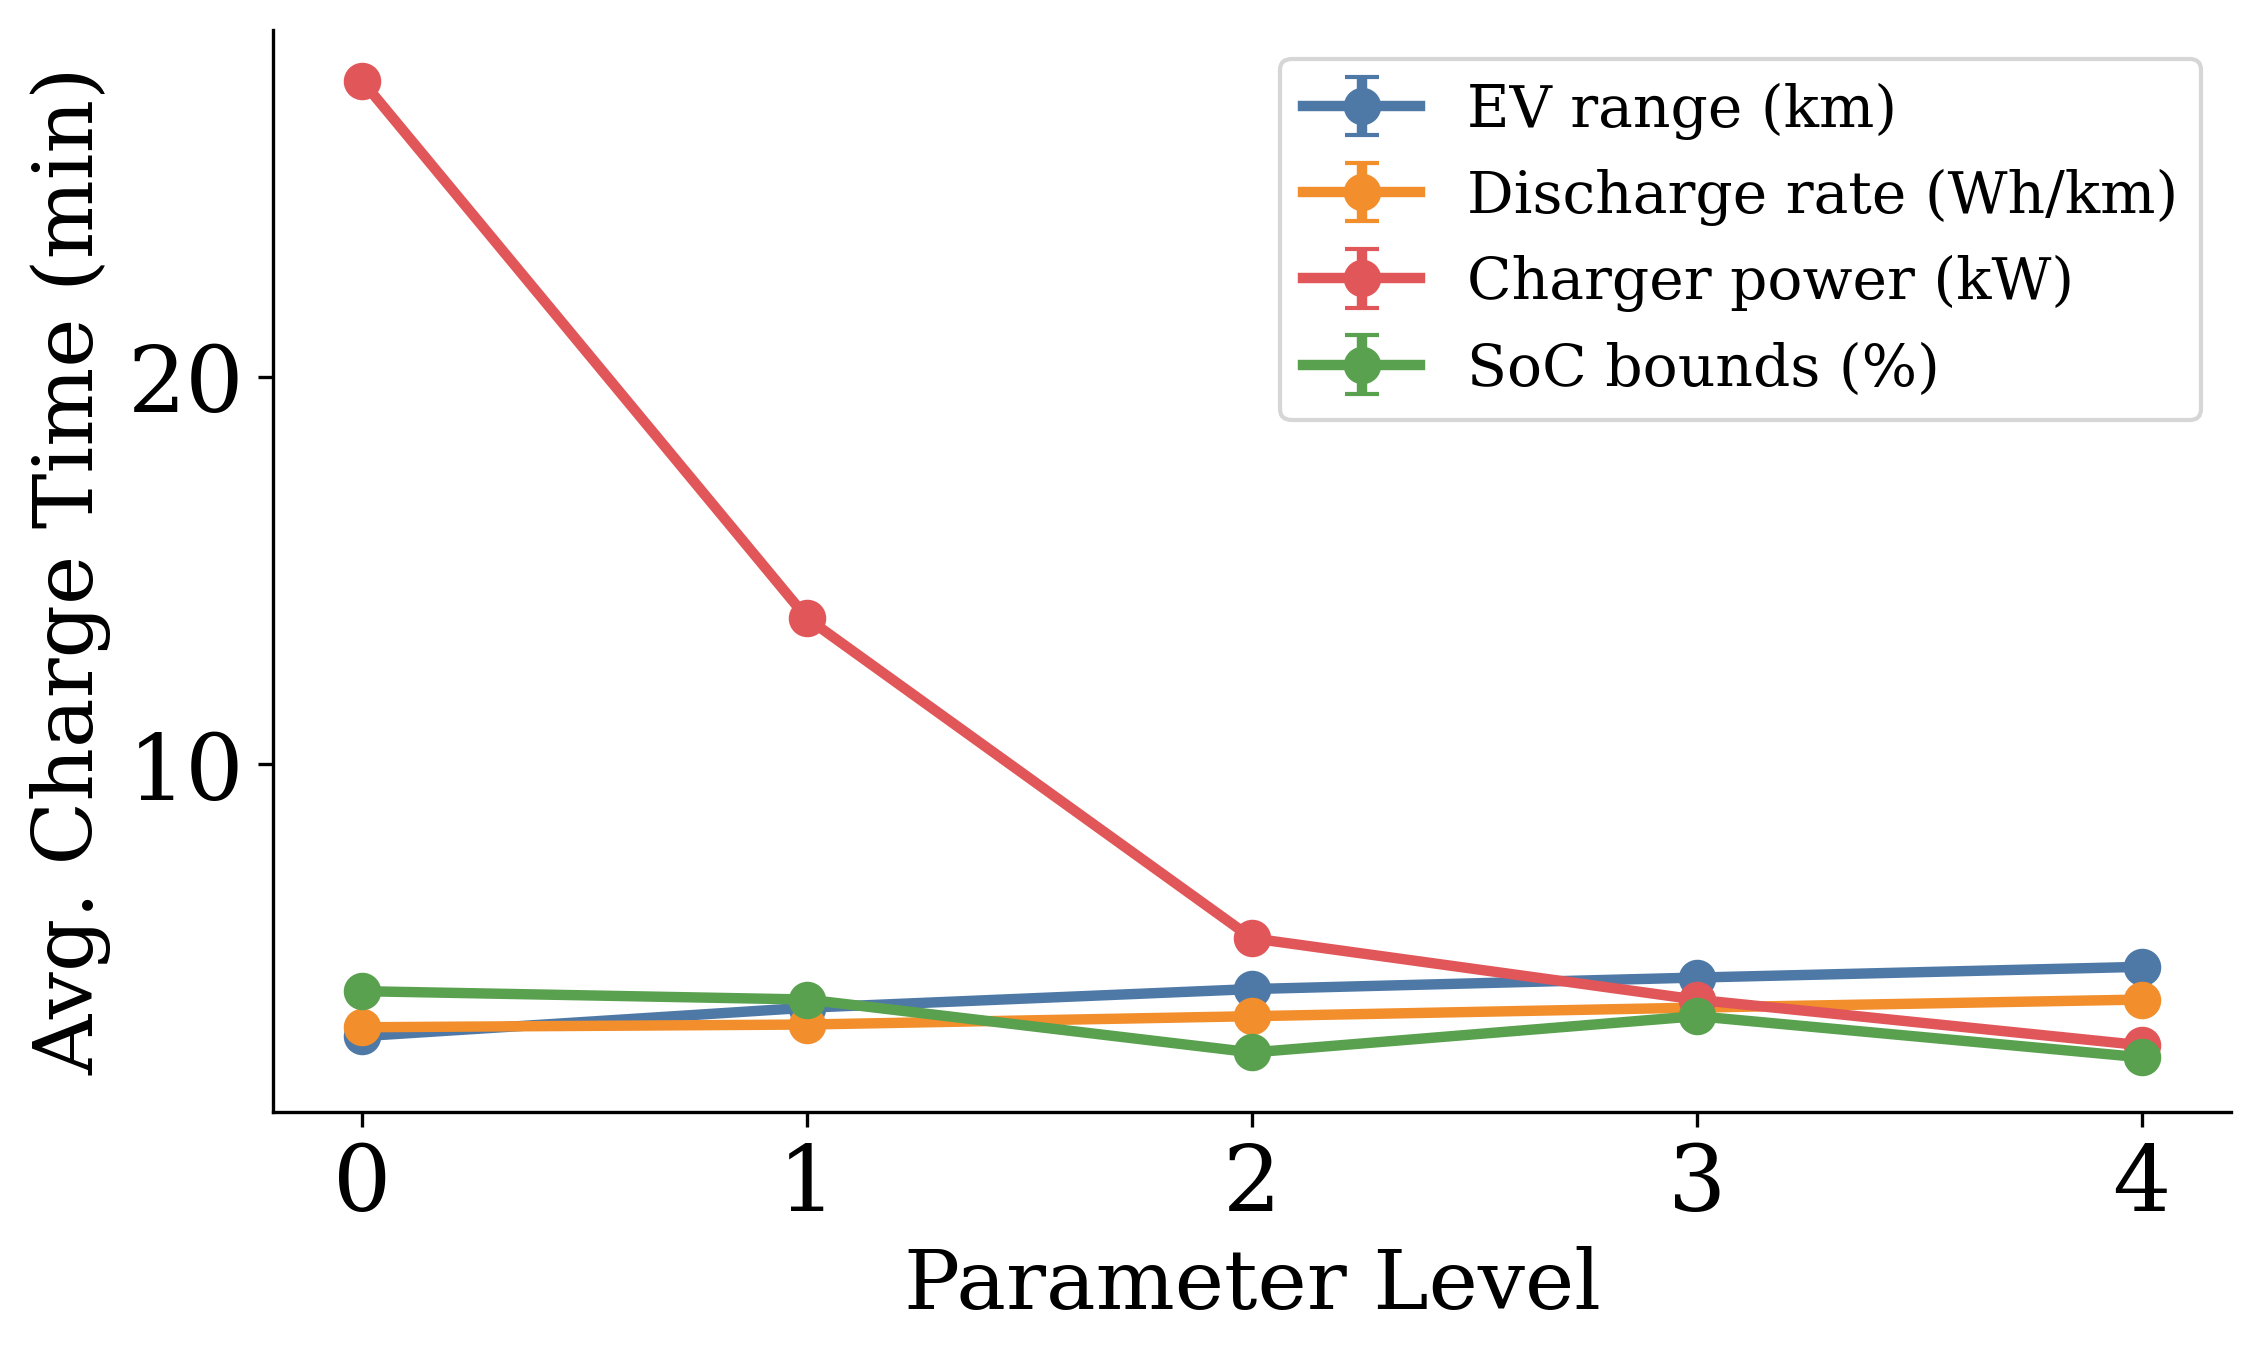
\includegraphics[width=\textwidth]{sensitivity_charge_time_tr.png}
    \caption{Average charge time per stop}
\end{subfigure}

\vspace{6pt}
\begin{subfigure}[t]{0.48\textwidth}
    \centering
    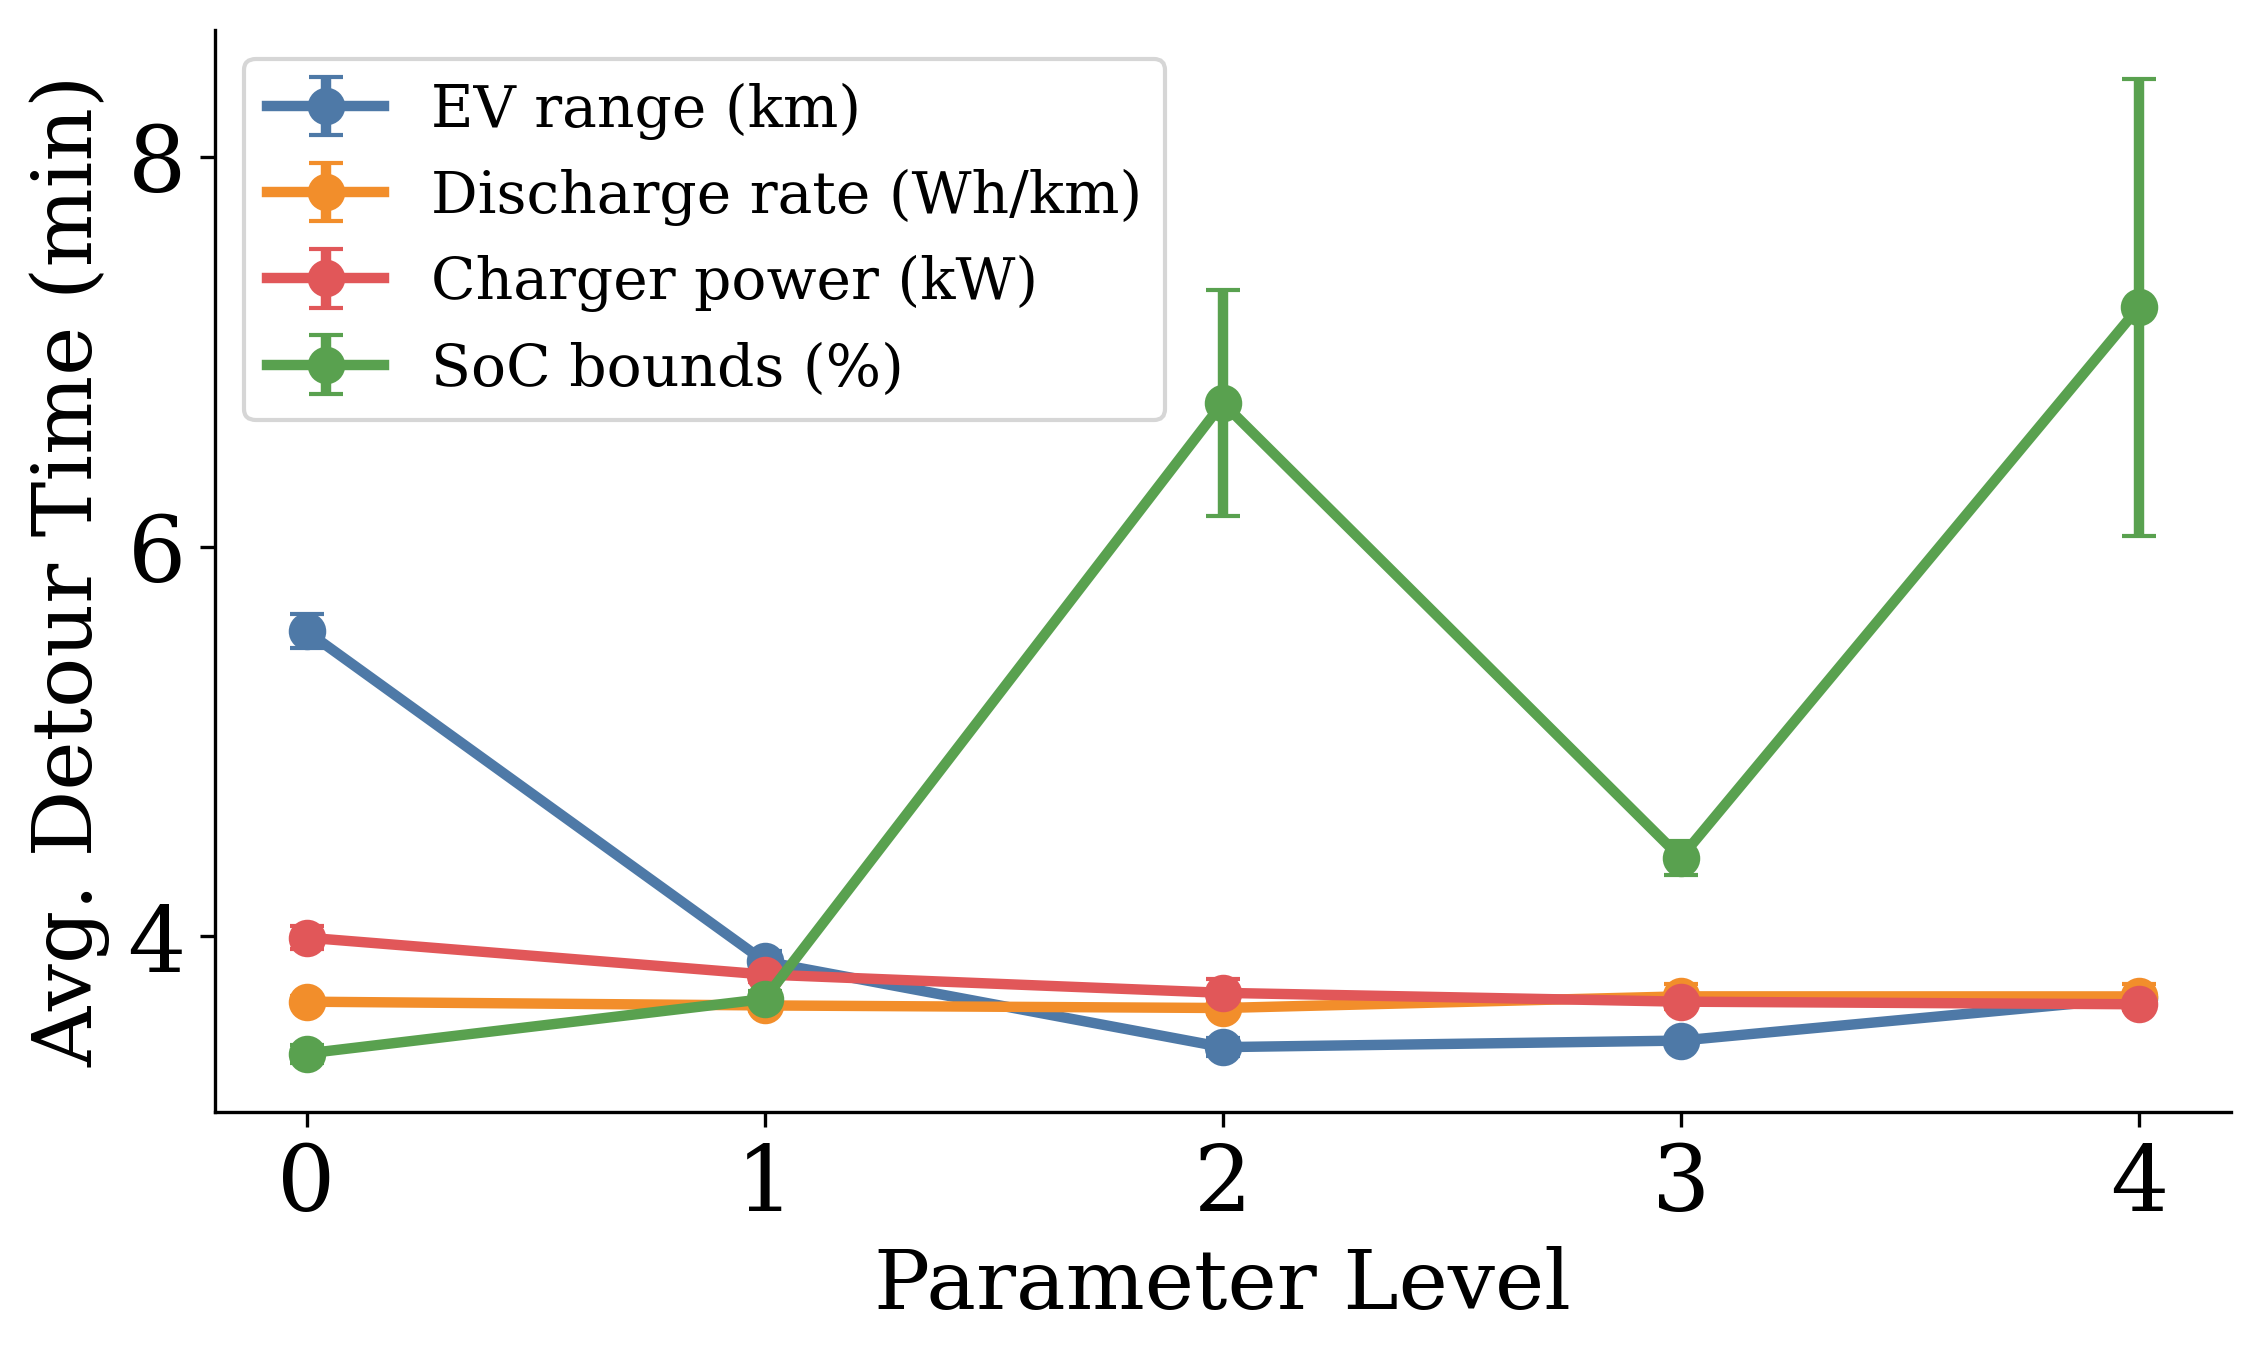
\includegraphics[width=\textwidth]{sensitivity_detour_time_tr.png}
    \caption{Average detour time per path}
\end{subfigure}
\hfill
\begin{subfigure}[t]{0.48\textwidth}
    \centering
    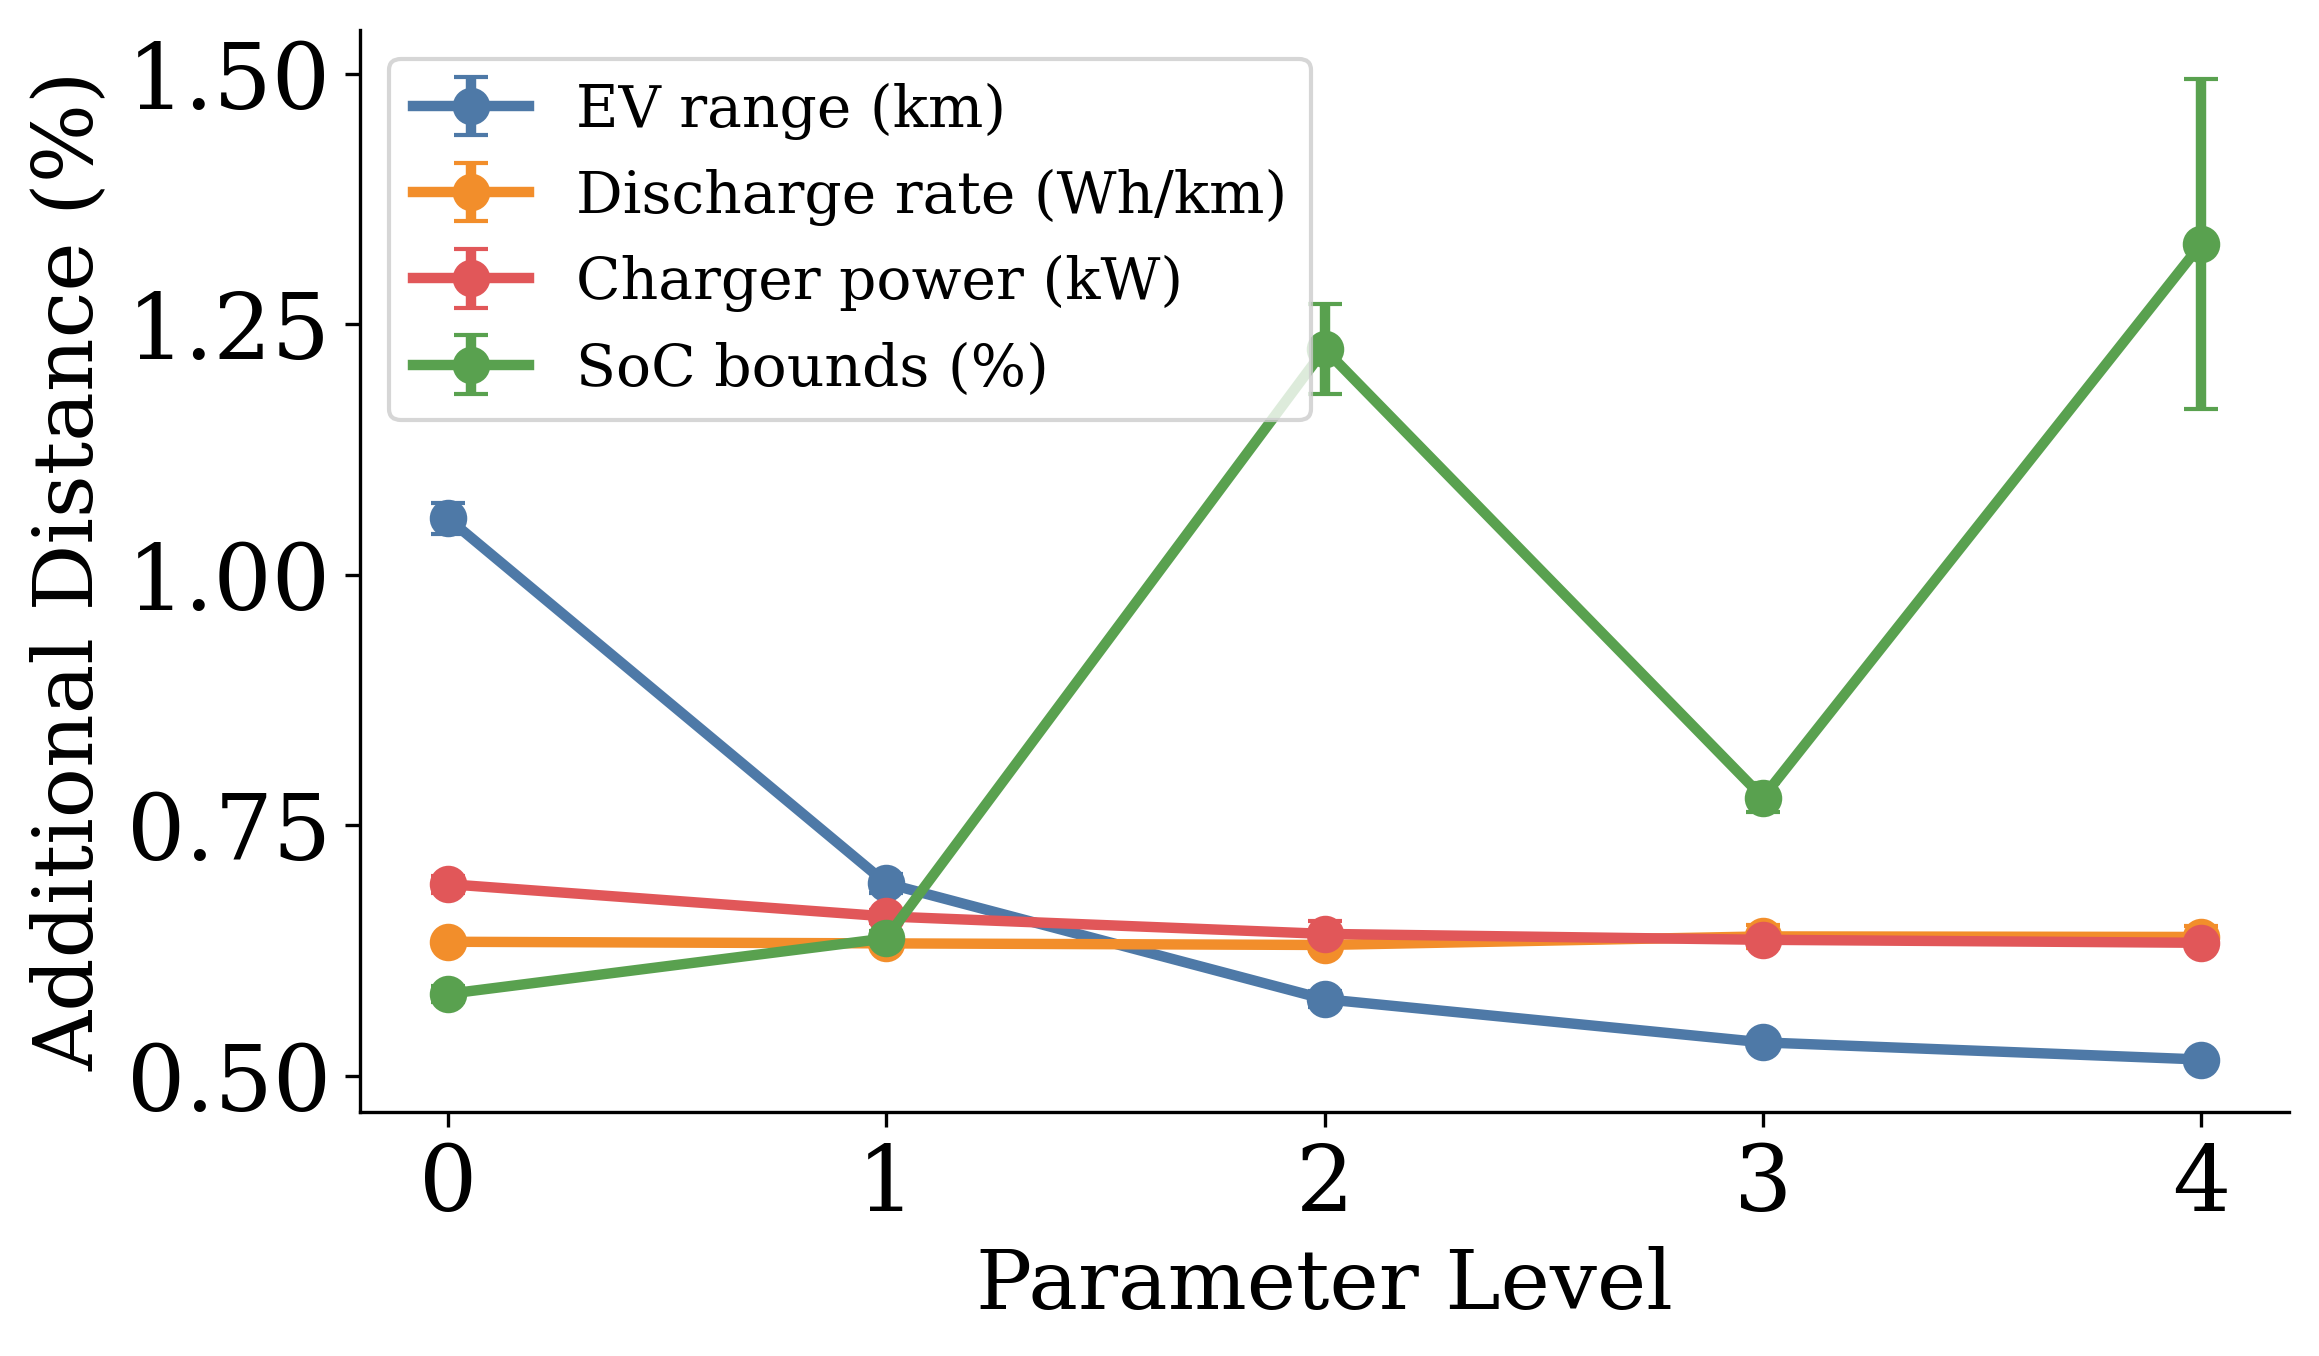
\includegraphics[width=\textwidth]{sensitivity_add_dist_tr.png}
    \caption{Additional travel distance}
\end{subfigure}
\caption{Charging operations across sensitivity sweeps. Each line represents one parameter sweep; markers show mean values over 10 replications with $\pm$1 standard deviation error bars.}
\label{fig:sensitivity_ops}
\end{figure*}

% =============================================================================
\section{Conclusion}\label{sec:conclusion}
% =============================================================================

This paper assessed the readiness of T\"{u}rkiye's EV charging infrastructure for intercity personal vehicle travel by applying the DAG-based scheduling framework of \citet{cokyasar2026electrification} to the country's full intercity highway network. The analysis covered 9,641 EPDK-licensed charging stations, 3 million synthetic origin-destination trips derived from KGM traffic statistics and T\"{U}\.{I}K demographic data, and an intercity road network of 31,286 nodes and 55,236 links constructed from OpenStreetMap. Eight case study scenarios crossing four charger power levels (5, 22, 50, and 350~kW) with two plug-count assumptions (5 and 50 per station) were evaluated at full electrification, supplemented by a 200-run sensitivity analysis over EV range, discharge rate, charger power, and SoC operating bounds.

Four principal findings emerged. First, T\"{u}rkiye's charging network achieves 100\% intercity trip feasibility when vehicles can utilize their full battery capacity (SoC window of 10--100\%), but feasibility collapses to 0.3\% under a conventional 20--80\% operating range, revealing that infrastructure adequacy hinges critically on how much of the battery is usable between stops. Second, EVs are already operationally cheaper than ICE vehicles for intercity travel in T\"{u}rkiye, with Tier~1 savings of 23--26\% across all scenarios, driven by the country's favorable fuel-to-electricity price ratio (gasoline at 50~TL/liter vs.\ electricity at 13~TL/kWh). Third, the economic viability of the infrastructure investment depends on plug density: with 50 plugs per station, the amortized infrastructure cost pushes Tier~3 savings negative ($-15$\%), while with 5 plugs per station, Tier~3 remains positive ($+$7--8\%), framing a tangible tradeoff between congestion resilience and cost recovery. Fourth, discharge rate (energy efficiency) is the dominant sensitivity lever (12.5 percentage points of Tier~2 swing), exceeding the influence of EV range (5.9~pp), SoC bounds (2.0~pp), and charger power (0.0~pp at low adoption), suggesting that incentivizing energy-efficient vehicle models will yield larger cost competitiveness gains than infrastructure upgrades alone.

These results carry several practical implications for T\"{u}rkiye's charging infrastructure policy. The SoC feasibility cliff suggests that EPDK and KGM should prioritize filling charger coverage gaps on long intercity corridors, particularly in eastern and central Anatolia, where stretches between consecutive stations exceed the usable SoC range under conservative operating assumptions. The favorable Tier~1 economics indicate that intercity EV travel is already cost-competitive at the operational level, strengthening the case for accelerating EV adoption incentives. The Tier~3 plug-density tradeoff informs station sizing decisions: deploying fewer plugs per station keeps infrastructure costs recoverable through user fees, while excess capacity, though beneficial for congestion, imposes a per-trip cost burden that may require public subsidy.

Several limitations should be noted. The scheduling framework assumes linear charging at a constant rate to the target SoC at every stop; incorporating nonlinear taper curves and partial charging would improve fidelity. Detour distances are approximated as Manhattan distances at a constant speed rather than computed as actual road distances, and each vehicle accesses only its nearest station. The synthetic demand, while calibrated to aggregate intercity traffic volumes, does not capture temporal peaking patterns, seasonal variation, or route-choice heterogeneity present in observed travel data. The plug-count assumption (5 or 50 per station uniformly) does not reflect the heterogeneity of actual station capacities across T\"{u}rkiye's charging network. The capacity resolution heuristic provides no optimality guarantee, though the FIFO fallback ensures feasibility for every schedulable vehicle.

Future work should address these limitations along several directions. Integrating observed intercity travel data, such as KGM automatic traffic counter records or mobile phone origin-destination matrices, would replace the synthetic demand with empirically grounded trip patterns. Coupling the scheduling framework with a charger siting optimization model, using the congestion and detour cost outputs as feedback signals, could inform strategic placement of new stations in underserved corridors. Extending the analysis to commercial vehicle fleets (trucks, intercity buses) and to heterogeneous charger types within a single network would broaden the policy relevance. Finally, a comparative analysis across multiple emerging EV markets using the same framework could reveal how infrastructure readiness varies with geography, energy prices, and network topology.

\section*{Acknowledgments}
This material is based on work supported by the U.S. Department of Energy (DOE), Office of Science, under contract number DE-AC02-06CH11357. This report and the work described were sponsored by the DOE Transportation Technologies Office (TTO) under the Pathways to Affordable, Convenient, and Efficient Regional Mobility, an initiative of the Energy Efficient Mobility Systems (EEMS) Program. Erin Boyd, a DOE Office of Critical Minerals and Energy Innovation (CMEI) manager, played an important role in establishing the project concept, advancing implementation, and providing guidance.

\noindent\textbf{Author Contributions:} T. Cokyasar conducted study conception, design, data collection, analysis, and preparation. The author(s) reviewed and approved the manuscript.\\
\noindent\textbf{AI Use:} During the preparation of this manuscript, the author(s) used Claude Opus 4.6 and Claude Sonnet 4.6 through ARGO AI platform at Argonne National Laboratory to improve language, spelling, readability, literature review, coding, and result analysis. After using these tools, the author(s) meticulously reviewed and edited the entire text, code, and references (including manuscripts and all online links) and take full responsibility for the content of the publication.\\
\noindent\textbf{Conflict of Interest:} None declared.\\
\noindent\textbf{ORCID:}
\def\orcid#1{\kern .08em\href{https://orcid.org/#1}{
\includegraphics[keepaspectratio,width=0.7em]{orcidlogocol.png}}}
Taner Cokyasar \orcid{0000-0001-9687-6725} \url{https://orcid.org/0000-0001-9687-6725}\\